% Journal paper for Neurocomputing (Elsevier), elsarticle template.
% Source of the numbers: reports/Latex_report/v1_mnist_fashion_mnist_report/combined_report_v2.tex and outputs/.
% Build: pdflatex, bibtex, pdflatex, pdflatex.

\documentclass[preprint,review,12pt]{elsarticle}

\usepackage{graphicx}
\usepackage{booktabs, array, multirow}
\usepackage{amsmath, amssymb}
\usepackage{enumitem}
\usepackage{placeins}
\usepackage{url}
\usepackage{lineno}
% DOIs in the bibliography contain underscores: make \path verbatim-like and \href plain text
\DeclareUrlCommand\path{\urlstyle{same}}
\providecommand{\href}[2]{#2}
\graphicspath{{Fig/}}
\setlist[itemize]{leftmargin=1.4em, itemsep=2pt}
\renewcommand{\topfraction}{0.9}
\renewcommand{\floatpagefraction}{0.7}
\newcolumntype{L}[1]{>{\raggedright\arraybackslash}p{#1}}
\newcolumntype{C}[1]{>{\centering\arraybackslash}p{#1}}

\journal{Neurocomputing}

\begin{document}

\begin{frontmatter}

\title{Post-Training Analysis and Novelty Detection Using Neural Network Self-Organizing Maps (NNSOM)}

\author[gwu]{Fyrooz Anika Khan\corref{cor1}}
\ead{f.khan1@gwmail.gwu.edu}
\author[gwu]{Nazish Atta}
\author[gwu]{Amir Hossein Jafari}
\affiliation[gwu]{organization={Data Science Program, The George Washington University},
            addressline={2127 G Street NW},
            city={Washington},
            postcode={20052},
            state={DC},
            country={USA}}
\cortext[cor1]{Corresponding author.}
% ORCID iDs are entered in Elsevier's submission system (Fyrooz Anika Khan: 0009-0001-4265-4040).

\begin{abstract}
Deep networks can be accurate yet fail systematically in ways that single-prediction explanations miss. This paper studies whether a self-organizing map (SOM), built with a modified training loop of the Neural Network Self-Organizing Map (NNSOM) library on the penultimate-layer features of a fixed LeNet-5 convolutional neural network (CNN), helps to analyze errors, detect novel inputs and guide retraining. The same pre-registered design, with chance-level controls and simple baselines, is applied to Modified National Institute of Standards and Technology (MNIST) digits (99.18\% test accuracy) and Fashion-MNIST (90.90\%). What works: classes form distinct map regions (purity 98.2\% and 89.3\%, against about 17\% for shuffled labels), and errors concentrate in a few cells where classes overlap, at 11.1 and 3.9 times their share. On unseen clothing classes, the map's quantization error scores higher than the network's confidence (+0.046 area under the receiver operating characteristic curve, AUROC), although the nearest-neighbor distance scores higher still. What does not: k-means ranks errors about as well, the network's confidence ranks them better, and the energy score detects Street View House Numbers (SVHN) images better on both datasets. Guided retraining reduces the MNIST hotspot error (11.4\% to 7.8\%), but least-confident images do about as well and the gain over random images is not significant across seeds; on Fashion-MNIST the gain is not significant. A curriculum that never reaches the hardest 60\% of the hard pool lowers accuracy. The SOM is most useful as an explanatory map that shows where, and between which classes, a network fails.
\end{abstract}

\begin{highlights}
\item Map regions separate classes: purity 98.2\% (MNIST), 89.3\% (Fashion-MNIST)
\item Errors cluster in few map cells, 11.1x and 3.9x their share of the data
\item Map quantization error beats confidence on unseen clothing classes (+0.046 AUROC)
\item Confidence and energy scores beat the map for error and far-novelty detection
\item Map-guided retraining cut MNIST hotspot errors 11.4\% to 7.8\%; confidence did as well
\end{highlights}

\begin{keyword}
Self-organizing map \sep post-training analysis \sep error analysis \sep novelty detection \sep guided retraining \sep convolutional neural network
\end{keyword}

\end{frontmatter}
% Line numbers start after the title page; on the title page they clash with the footnote and footer
\linenumbers

% ------------------------------------------------------------------------------------------------------------------------
\section{Introduction}\label{sec:intro}

Deep neural networks have achieved high accuracy on many benchmark tasks, yet they can still fail in unexpected ways once deployed. Knowing why a model fails is therefore as important as improving its average accuracy. Widely used explanation methods, such as saliency maps~\cite{simonyan2014saliency}, local interpretable model-agnostic explanations (LIME)~\cite{ribeiro2016lime} and SHapley Additive exPlanations (SHAP)~\cite{lundberg2017shap}, explain individual predictions. They show which input features influenced one output, but they do not show whether the errors of a model follow a pattern across a whole dataset.

In this paper, we use a self-organizing map (SOM)~\cite{kohonen1990som} to obtain a global, post-training view of a trained network. A SOM projects high-dimensional data onto a two-dimensional grid so that similar inputs are placed in nearby cells. We train a convolutional neural network (CNN), take the 84-dimensional vector that it computes for each image before its output layer (the \emph{embedding}), and train a SOM on these embeddings with the Neural Network Self-Organizing Map (NNSOM) library~\cite{jafari_nnsom}. The training loop of the library was modified (Section~\ref{sec:method}), and no other SOM package was used. The map is then applied to three tasks: \emph{error analysis} (where the errors fall on the map, and why), \emph{novelty detection} (flagging inputs that differ from the training data) and \emph{guided retraining} (choosing training images for augmentation, compared with random choice and with choice by the network's confidence).

We follow the questions ``what works, what does not, what works best, and why?'' and apply the complete pipeline to two datasets under one pre-registered design. The first is the Modified National Institute of Standards and Technology (MNIST) database of handwritten digits~\cite{lecun1998gradient}, on which the network makes very few errors. The second is Fashion-MNIST~\cite{xiao2017fashion}, a set of clothing images on which the same network makes about ten times as many errors. Novelty detection is also tested with the Street View House Numbers (SVHN) dataset~\cite{netzer2011reading}, which differs strongly from both. The study is limited to one network (LeNet-5) and to these two $28\times28$ grayscale datasets. All success criteria were specified before the test data were used, and every result is compared with a chance level or a simple baseline.

The main contributions of this paper are as follows.
\begin{itemize}
  \item A reusable pipeline (CNN $\rightarrow$ embeddings $\rightarrow$ SOM $\rightarrow$ error analysis, novelty detection and guided retraining) that runs without modification on both datasets.
  \item Evidence that classification errors concentrate in regions where classes overlap on the map, on both datasets and for three grid sizes, well beyond chance.
  \item A controlled comparison with simple baselines, which shows that, in our experiments, the network's own confidence detected errors and far out-of-distribution inputs better than the map, and that k-means clustering located errors about as well as the SOM.
  \item Two settings in which the SOM was useful: it scored higher than the network's confidence, on average, on unseen clothing classes (although the nearest-neighbor distance scored higher still), and on MNIST the training images it selected, once augmented, were followed by fewer errors in the affected regions (although least-confident images did about as well, and the gain over random images is not significant across seeds).
\end{itemize}

The remainder of this paper is organized as follows. Section~\ref{sec:related} reviews related work. Section~\ref{sec:method} describes the pipeline and the experimental protocol. Section~\ref{sec:results} reports what works, what does not and what works best. Section~\ref{sec:discussion} explains the results and states the limitations, and Section~\ref{sec:conclusion} concludes the paper.

% ------------------------------------------------------------------------------------------------------------------------
\FloatBarrier
\section{Related Work}\label{sec:related}

\subsection{Explaining individual predictions}
Saliency maps~\cite{simonyan2014saliency} highlight the pixels that most affect a class score, LIME~\cite{ribeiro2016lime} fits an interpretable local model around one prediction, and SHAP~\cite{lundberg2017shap} attributes a prediction to its input features. These methods answer the question ``why was this prediction made?''. We address a complementary question: where in the feature space do the errors concentrate?

\subsection{Self-organizing maps}
Kohonen's SOM~\cite{kohonen1990som} preserves the neighborhood structure of the data on a low-dimensional grid, and Vesanto and Alhoniemi~\cite{vesanto2000clustering} showed how the cells of a trained map can be clustered and evaluated. NNSOM~\cite{jafari_nnsom} provides the SOM implementation and quality measures used in this work. The Self-Organizing Map Variational Autoencoder (SOM-VAE)~\cite{fortuin2019somvae} and the Deep Embedded Self-Organizing Map (DESOM)~\cite{forest2021desom} learn the representation and the map jointly. We deliberately keep the network fixed, so that the contribution of the map can be assessed in isolation. SOMs and related topographic layouts have also been used to look inside trained networks: Krug et al.~\cite{krug2023topographic} arrange the neurons of a layer so that similar activations lie close together and use the resulting maps to spot errors and biases, Lee and Vijayan~\cite{lee2022generalization} use SOMs to study the internal codes of deep networks, d'Aquin~\cite{daquin2023concept} locates concept representations in layer activations with SOMs, and Braga et al.~\cite{braga2020batchsssom} train a semi-supervised SOM on CNN features of MNIST, Fashion-MNIST and SVHN. These works study representations or classify with the map; we instead use the map after training to locate the errors and novel inputs of a fixed classifier and test it against simple baselines.

\subsection{Discovering systematic errors}
Domino~\cite{eyuboglu2022domino} identifies data slices on which a model underperforms and describes them in natural language, and Spotlight~\cite{deon2022spotlight} searches the representation space for regions of high loss, and Zhang et al.~\cite{zhang2023diagnosing} use a shared image--text embedding to find high-error slices and correct them with language. Closer to our error-detection baselines, the trust score of Jiang et al.~\cite{jiang2018trust} measures how far a prediction agrees with a nearest-neighbor classifier in feature space, and Deep k-Nearest Neighbors~\cite{papernot2018dknn} uses the labels of neighboring training points in each layer to estimate confidence. Jiang et al.\ report that on high-dimensional data the trust score may give little or no gain over the model's confidence; our results for the SOM's cell error rate are similar (Table~\ref{tab:baselines}). These methods are closest to our error analysis. Our approach differs in two respects: it uses a topology-preserving map that gives a single, interpretable view of the feature space, and it tests every claim against chance and against simple baselines.

\subsection{Novelty and out-of-distribution detection}
Hendrycks and Gimpel~\cite{hendrycks2017baseline} proposed the maximum softmax probability as a baseline detector. The Out-of-DIstribution detector for Neural networks (ODIN)~\cite{liang2018odin} improves on it, Lee et al.~\cite{lee2018mahalanobis} use the Mahalanobis distance to class centroids, Liu et al.~\cite{liu2020energy} propose an energy score, Deep Support Vector Data Description (Deep SVDD)~\cite{ruff2018deep} learns a compact description of normal data, and Sun et al.~\cite{sun2022knn} use the distance to the nearest training features; Yang et al.~\cite{yang2024generalized} provide a survey. We also compare with Isolation Forest~\cite{liu2008isolation}, the One-Class Support Vector Machine (SVM)~\cite{scholkopf2001support} and autoencoder reconstruction error~\cite{sakurada2014autoencoder}. SOM quantization errors have been used to detect anomalies in multi-scale deep features of industrial images~\cite{li2021somad} and outliers in microscopy images of blood cells~\cite{rohrl2022outlier}; both are unsupervised detectors trained for that purpose, whereas we use the QE of a map built on a classifier's features as a post-hoc diagnostic and compare it with the classifier's own scores. Nalisnick et al.~\cite{nalisnick2019deep} showed that models of normal data can assign higher likelihood to unfamiliar images; in our experiments two detectors of normal data likewise rate SVHN images as more normal than the in-distribution images. For unseen classes we follow the open-set protocol of Neal et al.~\cite{neal2018open}, under which the maximum softmax probability is a strong baseline~\cite{vaze2022openset}. We do not claim that the SOM outperforms these methods; we test whether its measures provide a useful signal and show where failures occur.

\subsection{Hard examples, curriculum learning and augmentation}
Curriculum learning presents easy examples before hard ones~\cite{bengio2009curriculum}; Soviany et al.~\cite{soviany2022curriculum} survey how difficulty is measured and how the pace of introducing harder data is set. Online hard example mining~\cite{shrivastava2016ohem} instead concentrates training on the examples with the highest loss, and data augmentation~\cite{shorten2019augmentation} adds altered copies of training images. We use the SOM to decide which training images count as hard, and compare this choice with random images and with the network's least-confident images.

\subsection{Positioning of this work}
Previous work either explains individual predictions, learns the map jointly with the model, or detects novel inputs without locating the failures. In contrast, we apply a single SOM, trained on fixed features, to error analysis, novelty detection and guided retraining; we replicate the full design on two datasets; and we evaluate each claim against chance and simple baselines.

% ------------------------------------------------------------------------------------------------------------------------
\FloatBarrier
\section{Method}\label{sec:method}

Figure~\ref{fig:pipeline} shows the pipeline, which has four phases. Phase~1 trains and freezes the network, Phase~2 trains and analyzes the SOM, Phase~3 detects novel inputs, and Phase~4 uses the map to select images for retraining.

\begin{figure}[htbp]
\centering
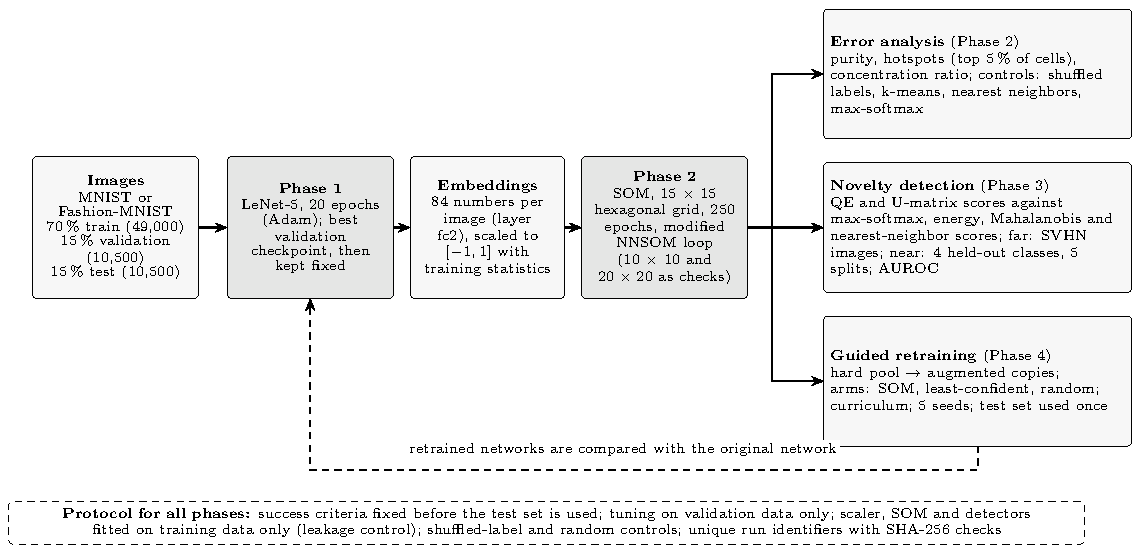
\includegraphics[width=\linewidth]{diagram_pipeline.pdf}
\caption{The pipeline of this study. A CNN is trained once and kept fixed, and the embeddings of its penultimate fully connected layer (fc2) are stored. A SOM is trained on the training embeddings, and the map is used for error analysis, novelty detection and guided retraining. The retrained networks are compared with the original one (dashed arrow). The protocol at the bottom applies to every phase. Diagram drawn as TikZ code written with Claude Sonnet 5.5 (Anthropic) and checked by the authors.}
\label{fig:pipeline}
\end{figure}

\subsection{Data and network (Phase 1)}

\subsubsection{Datasets}
MNIST has 70,000 handwritten digits in 10 classes, and Fashion-MNIST has 70,000 clothing images in 10 classes (T-shirt/top, Trouser, Pullover, Dress, Coat, Sandal, Shirt, Sneaker, Bag, Ankle boot); both are grayscale $28\times28$ images. Each dataset is split once into 70\% training (49,000 images), 15\% validation (10,500) and 15\% test (10,500), stratified by class with a fixed seed. Pixel values are scaled to $[0,1]$. As out-of-distribution data we use the 26,032 test images of SVHN~\cite{netzer2011reading}, converted to grayscale and resized to $28\times28$.

\subsubsection{Network}
LeNet-5~\cite{lecun1998gradient} is trained with Adam~\cite{kingma2015adam} (learning rate 0.001, weight decay 0.0001, learning rate multiplied by 0.1 every 10 epochs, batch size 64, 20 epochs, seed 42), keeping the checkpoint with the highest validation accuracy. LeNet-5 is the only architecture used. For every image, the 84 activations of the penultimate fully connected layer (fc2) are stored as the embedding, with the label, prediction and confidence; embeddings are rescaled to $[-1,1]$ using training statistics only.

\subsection{Self-Organizing Map (Phase 2)}

\subsubsection{Principle of the SOM}
A SOM is a competitive network of neurons arranged on a grid, each with a weight vector of the input dimension~\cite{kohonen1990som,hagan2014nnd_ch16}. For each input, the neuron with the closest weight vector wins; the winner and its grid neighbors then move towards the input, so that nearby cells come to represent similar inputs. We use the batch version of this rule~\cite{hagan2014nnd_ch26}, which needs no learning rate: after each pass, each weight vector is replaced by a weighted average of the embeddings whose winners lie in its neighborhood. NNSOM~\cite{jafari_nnsom} supplies the implementation, but we replaced its training loop with a modified one that recomputes the winning neuron of every embedding at each epoch (NNSOM 1.8.x selects the winners from the initial weights); no other SOM package was used. Figure~\ref{fig:som} illustrates these steps.

\begin{figure}[htbp]
\centering
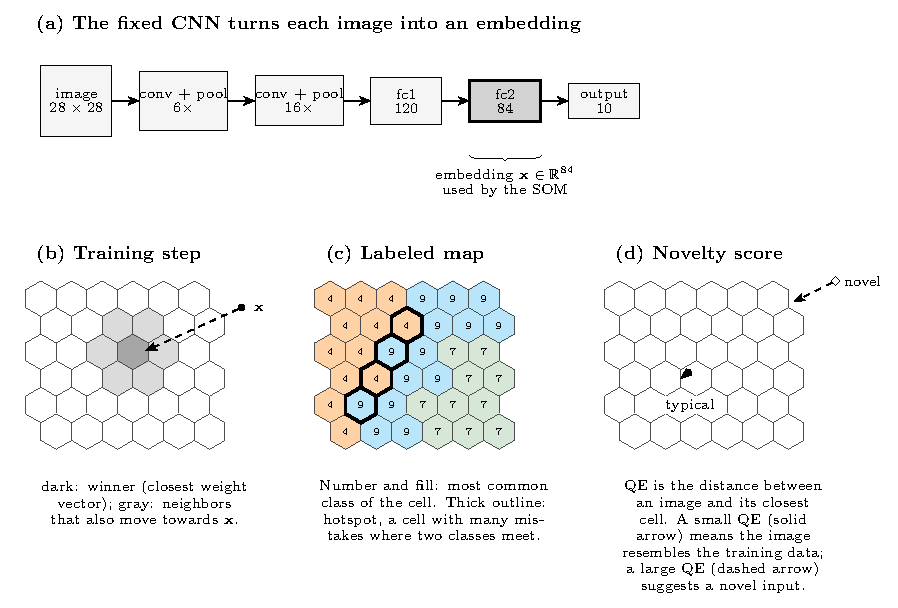
\includegraphics[width=0.95\linewidth]{diagram_som.pdf}
\caption{How the SOM works in this study. (a)~The fixed CNN turns each image into an 84-number embedding (layer fc2). (b)~The neuron whose weight vector is closest to the embedding wins, and the winner and its grid neighbors move towards the embedding. (c)~After training, each cell is labeled by its images: their most common class, how mixed the classes are, and how often the CNN is wrong there (hotspots). (d)~An image far from its best cell (large quantization error, QE) is unlike the training data. The grids are schematic (the class numbers are only an illustration); the real maps have $15\times15$ hexagonal cells. Redrawn after~\cite{hagan2014nnd_ch16,hagan2014nnd_ch26}. Diagram drawn as TikZ code written with Claude Sonnet 5.5 (Anthropic) and checked by the authors.}
\label{fig:som}
\end{figure}

\subsubsection{Training and map quality}
A hexagonal $15\times15$ SOM (225 cells) is trained with the modified loop on the 49,000 training embeddings for 250 epochs, with the neighborhood radius decreasing from 11 to 1 (seed 42). Each image is assigned to its best-matching unit (BMU). Map quality is measured by the quantization error (QE), which is the distance between an image and its BMU, and by the topographic error (TE1), which is the share of images whose two closest cells are not adjacent.

\subsubsection{Why the headline grid is $15\times15$}
Grids of $10\times10$, $15\times15$ and $20\times20$ were compared with a pre-specified procedure: ten maps per grid, with the error rate of each cell estimated on one half of the validation images and used to predict the errors in the other half, scored by the area under the receiver operating characteristic curve (AUROC)~\cite{fawcett2006roc}, over 200 half-splits. The first selection rule (ranks of QE, TE1 and occupancy) chose $20\times20$ on MNIST but chose $10\times10$ after the maps were retrained, so it was not stable; the $15\times15$ grid was adopted by project decision rather than by the rule. The equal-budget comparison, fixed before it was run, found no detectable difference between $15\times15$ and $20\times20$ on MNIST ($+0.001$, 95\% range $-0.100$ to $+0.089$, with only 92 mistakes; $+0.002$, $-0.101$ to $+0.101$ when the maps were trained again with the final code) and favored $15\times15$ on Fashion-MNIST ($-0.042$, $-0.077$ to $-0.008$, for $20\times20$ minus $15\times15$). We therefore report $15\times15$ as the headline map and use $10\times10$ and $20\times20$ as robustness checks; the error findings were the same on all three. A 20-trial Optuna search per grid~\cite{akiba2019optuna} (scored on validation QE and TE1 only) found no better setting for $15\times15$ on either dataset. SOMs on the earlier fully connected layer (fc1, 120 dimensions) were also compared with fc2 over 5 SOM seeds: fc2 located errors better (mean over 5 SOM seeds: AUROC 0.685 against 0.622 on MNIST, 0.815 against 0.760 on Fashion-MNIST), whereas fc1 detected SVHN better ($+0.005$ AUROC on MNIST, $+0.087$ on Fashion-MNIST).

\subsubsection{Error analysis}
For each cell we compute the purity (the share of images of its majority class) and the class entropy, and compare the overall purity with 1,000 random label permutations. Cells are ranked by the lower bound of the 95\% Wilson interval~\cite{wilson1927probable} of their error rate, and the top 5\% (11 cells) are the \emph{hotspots}. Hotspots are selected on one half of the validation images and evaluated on the other half with the \emph{concentration ratio}, the share of errors in the hotspots divided by the share of images in the hotspots. This is repeated over 100 random splits, each used in both directions (200 ratios), and compared with 200 permutations of the error labels.

\subsubsection{Baselines for error detection}
The same test is applied to k-means with 225 clusters, to the class impurity of the 15 nearest training embeddings, and to the network's maximum softmax probability~\cite{hendrycks2017baseline}.

\subsection{Novelty detection (Phase 3)}

\subsubsection{Far novelty}
The 10,500 validation images serve as normal data and the SVHN test images as novel data. We use the SOM's QE and the unified distance matrix (U-matrix) score (the mean distance between the BMU and its neighboring cells). The QE threshold is the 95th percentile of the training QE, fixed before any novel image was scored. On the same embeddings we compute the maximum softmax probability, the energy score~\cite{liu2020energy}, the Mahalanobis distance~\cite{lee2018mahalanobis}, the nearest-neighbor distance~\cite{sun2022knn}, Isolation Forest~\cite{liu2008isolation}, the One-Class SVM~\cite{scholkopf2001support} and an autoencoder~\cite{sakurada2014autoencoder}, with a random score as control. We report the AUROC, the area under the precision--recall curve (AUPR)~\cite{saito2015pr}, the false-positive rate at 95\% true-positive rate (FPR@95), and paired bootstrap intervals (2,000 resamples).

\subsubsection{Near novelty}
Because SVHN differs strongly from both datasets, we add a harder test following the open-set protocol~\cite{neal2018open}: in each of 5 class splits, drawn once at random and fixed before any run, a new LeNet-5 and a new $15\times15$ SOM are trained on 6 known classes, and the validation images of the other 4 classes are novel. Four hypotheses were fixed in advance: (H1) the SOM detects the unseen classes; (H2, primary) it outperforms the maximum softmax probability; (H3) it is no more than 0.01 AUROC worse than the maximum softmax probability, energy or Mahalanobis distance; (H4) it outperforms the nearest-neighbor distance. Each is tested with a 95\% $t$-interval over the five splits.

\subsection{Guided retraining (Phase 4)}

\subsubsection{Retraining algorithm}
(1)~Train the SOM on the training embeddings and keep it fixed. (2)~Rank its cells by the Wilson lower bound of their error rate on validation images and mark the 11 hotspots. (3)~Build the hard pool: a training image is hard if its cell is a hotspot, if its cell's purity is below 0.95, or if its distance to its BMU exceeds the 95th percentile. Two control pools of the same size and class composition are formed: random images, and the least-confident images (lowest maximum softmax probability). (4)~For each arm, add three augmented copies (small rotation, translation, scaling and shear) of every pool image to the training set, or order the pool for curriculum learning (the easy images and 10\% of the pool at first, a further 10\% every 5 epochs). (5)~Retrain a new LeNet-5 from scratch with the Phase~1 recipe for seeds 1 to 5, using the same seeds in every arm. (6)~Compare the arms on the hotspot test images and on all other test images with paired bootstrap intervals, and train a new SOM on each retrained network. Before training, the augmentation ranges had to pass a check: the baseline network may lose at most 2 percentage points of validation accuracy on augmented images. A hotspot-only pool, gradually paced variants and a re-analysis of the new maps were also evaluated. In the end-to-end comparison a test image is classified by the normally trained CNN (confusion matrix CF1) or by the CNN retrained with SOM-guided augmentation (CF2), averaged over the same 5 seeds.

Figure~\ref{fig:e2e} summarizes the end-to-end comparison.

\begin{figure}[htbp]
\centering
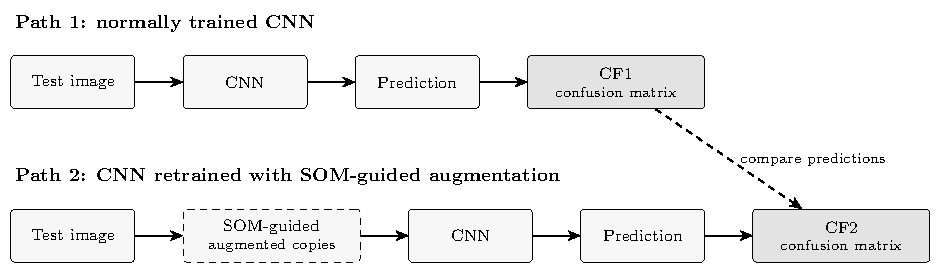
\includegraphics[width=0.95\linewidth]{diagram_cf1_cf2.pdf}
\caption{End-to-end comparison. The same test images are classified by the normally trained CNN (CF1) and by the CNN retrained with SOM-guided augmentation (CF2). The dashed box marks the retraining step of Phase 4. Diagram drawn as TikZ code written with Claude Sonnet 5.5 (Anthropic) and checked by the authors.}
\label{fig:e2e}
\end{figure}

\subsection{Figures}
All result figures are drawn by the project code from the saved experiment outputs. The hotspot outlines, hotspot labels and keys of the error maps (Figs.~\ref{fig:errormaps} and~\ref{fig:errormaps_f}) were added to the original figures by a script written with Claude Sonnet 5.5 (Anthropic) (\path{research_paper/scripts/label_error_maps.py}); the script reads the cell positions from the original figure and the labels from the saved validation results, and is included in the code repository.

\subsection{Experimental protocol}

\begin{itemize}
  \item \textbf{Pre-registration.} Success criteria, thresholds, numbers of splits and permutations, and seeds were recorded before the corresponding results were seen; for Phase 4 the protocol was time-stamped with a Secure Hash Algorithm 256 (SHA-256) hash before the test set was opened. The Fashion-MNIST protocol reproduced the MNIST design and was written before any Fashion-MNIST data were loaded.
  \item \textbf{Leakage control.} The scaler, the SOM, k-means, the nearest-neighbor reference set, the novelty detectors and the QE threshold are fitted on training embeddings only, and all Phase~2 and Phase~3 statistics are computed on validation images. The test set was used only to evaluate the baseline network and once in the final Phase~4 evaluation; no setting was selected on it. SVHN images were used only for scoring, and in the near-novelty experiment the held-out classes were never used for training, checkpoint selection, fitting or threshold setting. The validation set was also used to select the network checkpoint, so it is not entirely independent of model development.
  \item \textbf{Uncertainty and controls.} Accuracies have Wilson intervals; differences have paired bootstrap intervals over images or $t$-intervals over 5 seeds; map statistics are compared with permutation controls.
  \item \textbf{Fair comparisons.} All retraining arms use the same data, recipe, number of added images and seeds. Criteria that were not met are reported as such, and none was changed after the test evaluation. Comparisons designed after earlier results were known (the equal-budget baseline comparison, the classical novelty detectors, the embedding-length diagnostics and the seed-level interval below) are labeled exploratory.
  \item \textbf{Reproducibility.} Each run has a unique identifier and records the SHA-256 hashes of its inputs; completed runs are never overwritten.
\end{itemize}

% ------------------------------------------------------------------------------------------------------------------------
\FloatBarrier
\section{Results: what works, what does not, and what works best}\label{sec:results}

\subsection{Baseline networks}

LeNet-5 reaches a test accuracy of 99.18\% (95\% Wilson interval 98.99--99.34) on MNIST and 90.90\% (90.33--91.43) on Fashion-MNIST, with macro-F1 of 0.9918 and 0.9089. It makes 92 validation mistakes on MNIST and 876 on Fashion-MNIST, and its mean confidence is 0.997 when right and 0.833 when wrong on MNIST (0.942 and 0.686 on Fashion-MNIST). On Fashion-MNIST, confusions among T-shirt/top, Pullover, Coat and Shirt make up 638 of the 956 test mistakes (67\%), and Shirt is the weakest class (F1 0.746).

\subsection{What works: the map shows where errors concentrate}

Table~\ref{tab:som} and Figs.~\ref{fig:errormaps} and~\ref{fig:errormaps_f} summarize the maps. On both datasets the classes occupy distinct regions, far beyond chance (purity 98.2\% and 89.3\%, against 17.4\% and 17.3\% with shuffled labels), and the errors concentrate in a few cells where classes overlap: held-out hotspots hold 11.1 (MNIST) and 3.9 (Fashion-MNIST) times their share of the errors, against about 1.0 under label permutation. The same holds on the $10\times10$ and $20\times20$ maps (ratios 10.5 and 13.4 on MNIST, 3.81 and 3.81 on Fashion-MNIST). The error rate of a cell is strongly related to its class mixture (Spearman $-0.81$ and $-0.95$ with purity). The ratio cannot exceed one divided by the error rate (about 114 on MNIST and 12 on Fashion-MNIST), so the two ratios are not comparable.

\begin{table}[htbp]
\centering
\caption{SOM structure and error concentration (validation images, $15\times15$ map).}
\label{tab:som}
\small
\begin{tabular}{L{0.52\textwidth}C{0.17\textwidth}C{0.17\textwidth}}
\toprule
\textbf{Measure} & \textbf{MNIST} & \textbf{Fashion-MNIST} \\ \midrule
Quantization error (training) & 1.041 (1.039) & 0.899 (0.915) \\
Topographic error TE1 & 6.18\% & 5.37\% \\
Purity (with shuffled labels) & 98.2\% (17.4\%) & 89.3\% (17.3\%) \\
Cells with purity below 95\% & 44 & 121 \\
SOM hotspot concentration ratio, held out (spread over half-splits) & 11.1 (6.1--17.6) & 3.9 (3.2--4.4) \\
k-means hotspot concentration ratio (median; range over 10 seeds) & 5.6 (4.6--6.1) & 4.0 (3.7--4.5) \\
Chance level of the ratio & about 1.0 & about 1.0 \\
Spearman, cell error rate vs.\ purity & $-0.810$ & $-0.946$ \\
Spread over 10 retrained maps (standard deviation, SD): purity / TE1 & 0.12 / 0.28 points & 0.18 / 0.45 points \\ \bottomrule
\end{tabular}

\par\vspace{3pt}
{\footnotesize\raggedright All label-shuffle tests give $p=0.001$ (purity) or $p\le 0.005$ (hotspots, Spearman; 0.005 is the smallest value 200 shuffles allow). The bracketed range of the concentration ratio is the 2.5th to 97.5th percentile of 200 half-split ratios (100 random splits, each used in both directions); it is a spread over half-splits, not a confidence interval.\par}
\end{table}

\begin{figure}[htbp]
\centering
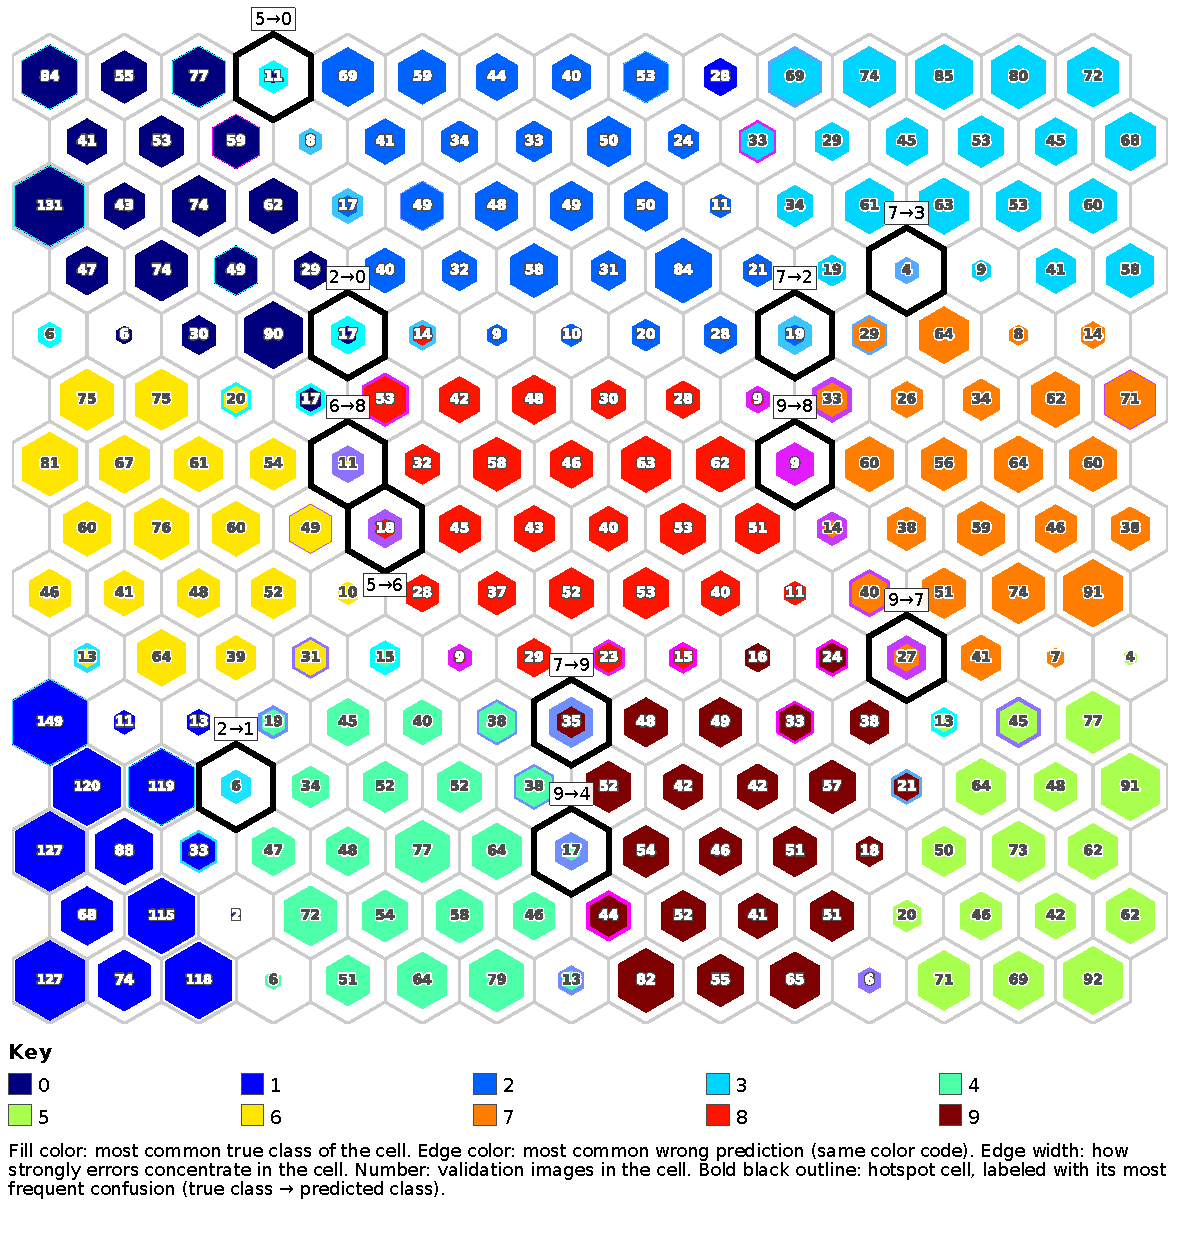
\includegraphics[width=0.85\linewidth,height=0.62\textheight,keepaspectratio]{error_map_mnist_labeled.pdf}
\caption{Validation error map of the $15\times15$ SOM on MNIST. Each hexagon is one cell; the fill color is the most common true class of its images and the edge color is the most common wrong prediction (same color code, see the key below the map). The number in a cell is the count of validation images in it. Thick outlines mark the 11 hotspot cells; each label gives the most frequent confusion in that cell (true class $\rightarrow$ predicted class). The frequent confusions are 4 predicted as 9, 5 as 0 and 9 as 4, and the hotspot images suggest shared strokes between 4 and 9, between 7 and 9, and among 5, 6 and 8 (a hypothesis, not a tested result).}
\label{fig:errormaps}
\end{figure}

\begin{figure}[htbp]
\centering
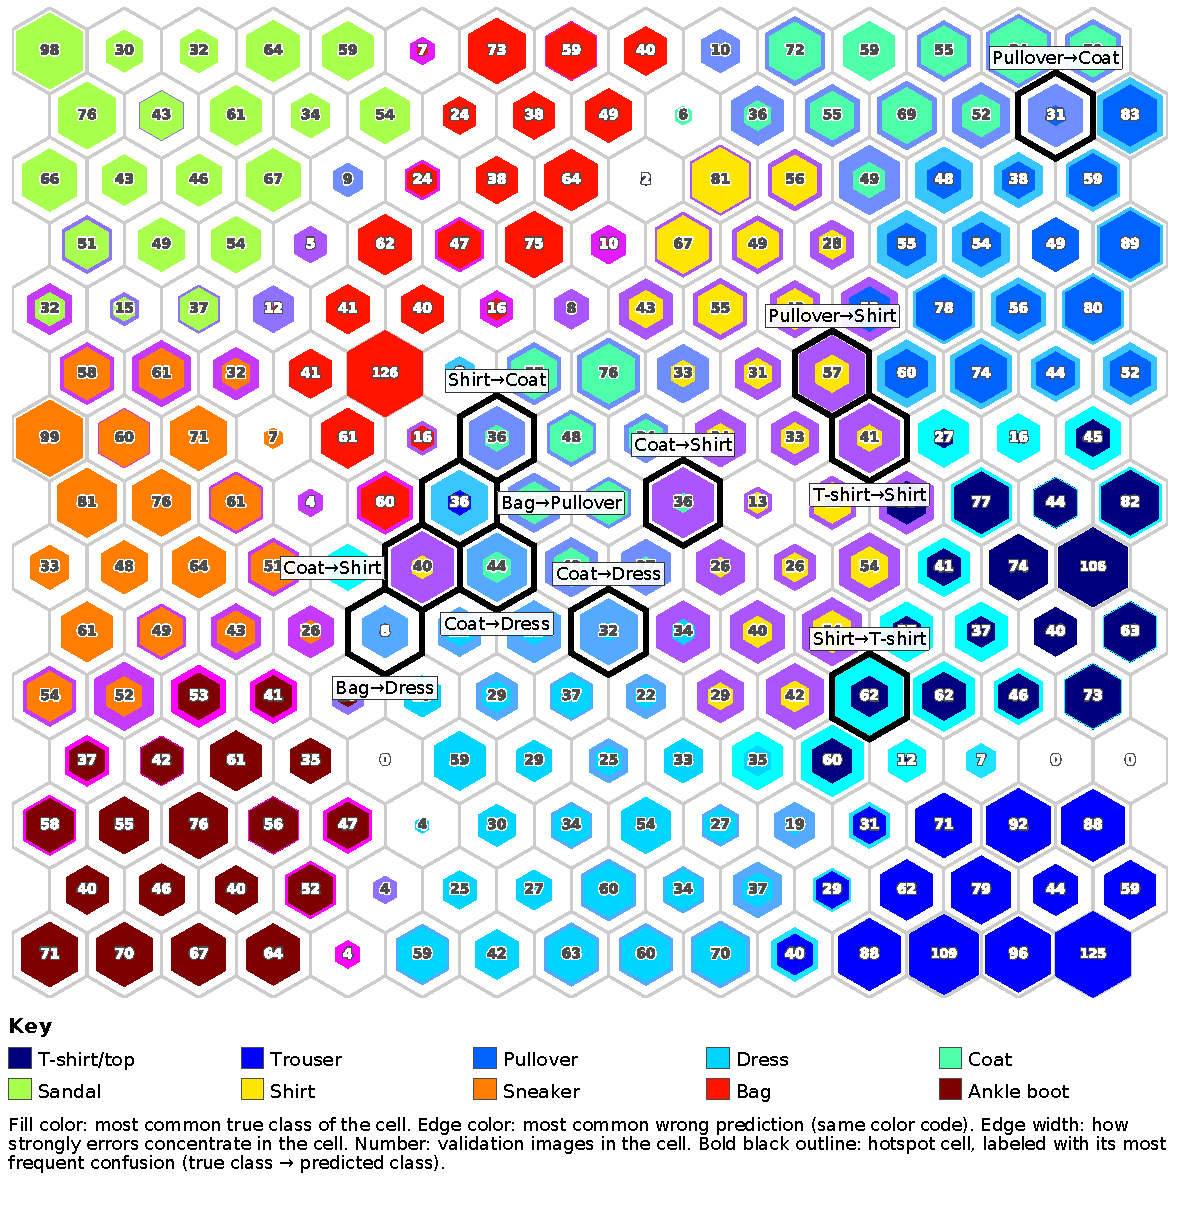
\includegraphics[width=0.85\linewidth,height=0.62\textheight,keepaspectratio]{error_map_fashion_mnist_labeled.pdf}
\caption{Validation error map of the $15\times15$ SOM on Fashion-MNIST, drawn as in Fig.~\ref{fig:errormaps}. Most hotspots mix Shirt, T-shirt/top, Pullover, Coat and Dress.}
\label{fig:errormaps_f}
\end{figure}

The map also shows the nature of the errors. On MNIST each frequent confusion lies in four or five cells, mostly among the cells of the predicted digit. On Fashion-MNIST each frequent confusion spreads over 24 to 27 cells, and in eight of the eleven hotspot cells the most frequent confusions are among upper-body garments (Coat with Shirt or Dress, Pullover with Coat or Shirt, Shirt with T-shirt/top); the other three are small cells that also contain bags resembling garments. At $28\times28$ pixels a collar, buttons or sleeve length occupy only a few pixels. Figures~\ref{fig:hotspot_mnist} and~\ref{fig:hotspot_fashion} (Appendix~A) show one representative error per hotspot (the one farthest from its cell): on MNIST they are ambiguous or atypical handwriting, six of the eleven with a confidence above 0.85, and on Fashion-MNIST mostly garments that resemble a neighboring class. These interpretations of the hotspot images are hypotheses, not tested results.



\subsection{What does not work: the SOM as an error or novelty detector}

\subsubsection{Error detection}
Table~\ref{tab:baselines} compares the SOM's cell error rate with simple baselines on the same embeddings. K-means clustering ranks the errors about as well as the SOM, and the network's own confidence ranks them better. The concentration ratios are similar on Fashion-MNIST (k-means 4.0, SOM 3.9). On MNIST the SOM's ratio is higher (11.1 against 5.6, Table~\ref{tab:som}), but its hotspots are smaller (1.6\% of the images against 3.8\%) and hold a slightly smaller share of the mistakes (18.1\% against 20.4\%, Table~\ref{tab:baselines}). Because the ratio rises as hotspots shrink, this difference reflects hotspot size rather than stronger concentration. The same-budget check in the table is exploratory.

\begin{table}[htbp]
\centering
\caption{Error detection by the SOM and simple baselines (validation images).}
\label{tab:baselines}
\small
\begin{tabular}{L{0.33\textwidth}C{0.1\textwidth}C{0.14\textwidth}C{0.1\textwidth}C{0.14\textwidth}}
\toprule
 & \multicolumn{2}{c}{\textbf{MNIST (92 mistakes)}} & \multicolumn{2}{c}{\textbf{Fashion-MNIST (876)}} \\
\textbf{Method} & \textbf{AUROC} & \textbf{Mistakes caught} & \textbf{AUROC} & \textbf{Mistakes caught} \\ \midrule
SOM cell error rate ($15\times15$) & 0.685 & 18.1\% & 0.811 & 13.7\% \\
k-means cell error rate (225) & 0.693 & 20.4\%$^*$ & 0.812 & 15.8\%$^*$ \\
15-nearest-neighbor impurity & 0.874 & 48.7\% & 0.876 & 21.1\% \\
Network max-softmax confidence & \textbf{0.981} & \textbf{53.3\%} & \textbf{0.906} & \textbf{21.9\%} \\ \bottomrule
\end{tabular}

\par\vspace{3pt}
{\footnotesize\raggedright ``Mistakes caught'': share of mistakes among the images flagged when every method flags the same share as the SOM's hotspots (MNIST 1.6\%, Fashion-MNIST 3.5\%); $^*$k-means flags its own hotspot share (3.8\% and 4.0\%).\par}
\end{table}

\subsubsection{Far novelty (SVHN)}
Table~\ref{tab:far} shows that the SOM's QE detects SVHN images on both datasets, strongly on MNIST (AUROC 0.981) and weakly on Fashion-MNIST (0.789), but the energy score and the maximum softmax probability are better on both. QE is slightly better than the nearest-neighbor distance on MNIST ($+0.005$, $+0.002$ to $+0.007$) and than the Mahalanobis distance on both datasets, and it is worse than the energy score by 0.019 (MNIST) and 0.193 (Fashion-MNIST). The fixed QE threshold catches 96.2\% of SVHN images on MNIST but only 3.0\% on Fashion-MNIST, where it flags a smaller share of SVHN than of normal images. Isolation Forest and the autoencoder rate SVHN as more normal than the in-distribution data on at least one dataset, consistent with earlier findings for models of normal data~\cite{nalisnick2019deep}.

\begin{table}[htbp]
\centering
\caption{Far novelty detection against SVHN (10,500 validation images against 26,032 SVHN test images).}
\label{tab:far}
\small
\begin{tabular}{L{0.42\textwidth}C{0.1\textwidth}C{0.1\textwidth}C{0.1\textwidth}C{0.1\textwidth}}
\toprule
 & \multicolumn{2}{c}{\textbf{MNIST}} & \multicolumn{2}{c}{\textbf{Fashion-MNIST}} \\
\textbf{Novelty score} & \textbf{AUROC} & \textbf{FPR@95} & \textbf{AUROC} & \textbf{FPR@95} \\ \midrule
Energy & \textbf{0.9998} & 0.0004 & \textbf{0.982} & 0.063 \\
Maximum softmax probability & 0.9985 & 0.008 & 0.884 & 0.307 \\
SOM quantization error (QE) & 0.981 & 0.045 & 0.789 & 0.420 \\
Nearest-neighbor distance ($k=5$) & 0.977 & 0.059 & 0.864 & 0.314 \\
SOM U-matrix score & 0.970 & 0.070 & 0.812 & 0.253 \\
One-Class SVM & 0.960 & 0.179 & 0.734 & 0.634 \\
Mahalanobis distance & 0.776 & 0.313 & 0.713 & 0.454 \\
Isolation Forest & 0.238 & 0.872 & 0.266 & 0.934 \\
Autoencoder (raw inputs) & 0.008 & 0.9999 & 0.583 & 0.744 \\ \bottomrule
\end{tabular}

\par\vspace{3pt}
{\footnotesize\raggedright One network and one map per dataset. FPR@95: false-positive rate at 95\% true-positive rate, i.e. the share of normal images flagged when 95\% of SVHN is caught. A random score gives AUROC 0.505 and label shuffles give 0.500. The classical detectors are exploratory.\par}
\end{table}

Figure~\ref{fig:umatrix} shows the U-matrices on which the U-matrix score is based.

\begin{figure}[htbp]
\centering
\begin{minipage}[c]{0.46\linewidth}\centering
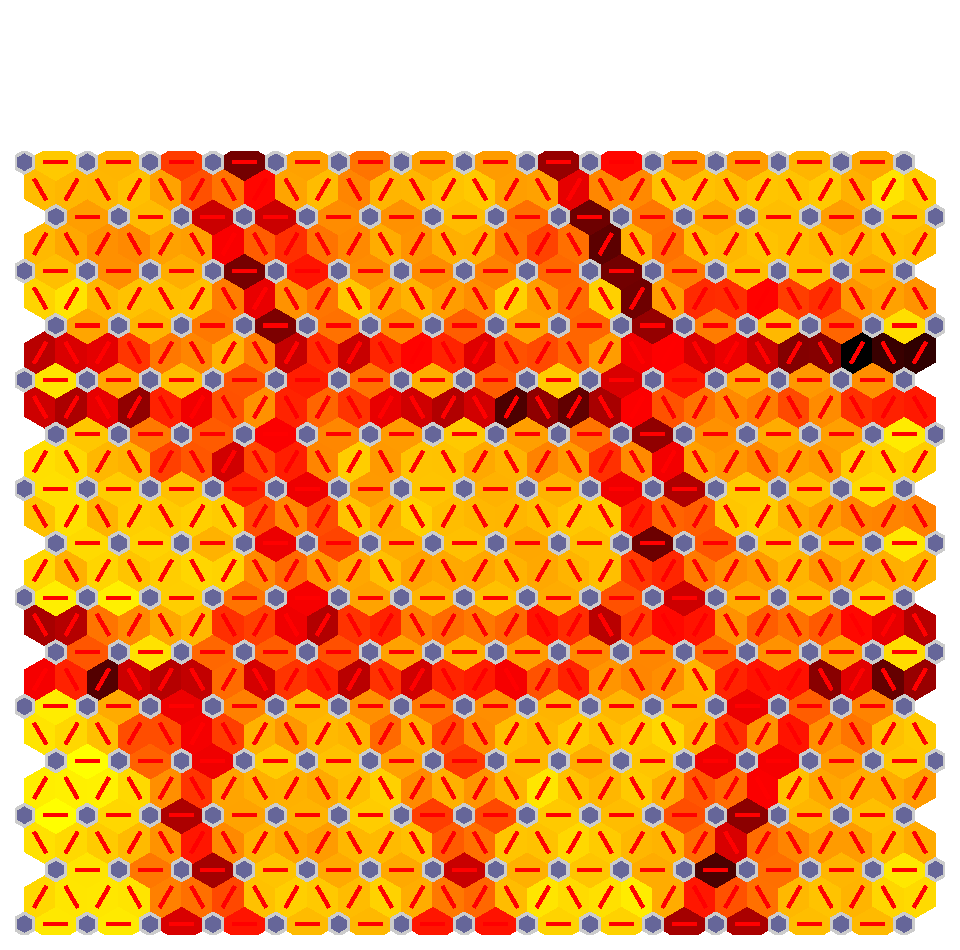
\includegraphics[width=\linewidth,keepaspectratio]{mnist_p2_u_matrix.pdf}\\{\small (a) MNIST}
\end{minipage}\hfill
\begin{minipage}[c]{0.46\linewidth}\centering
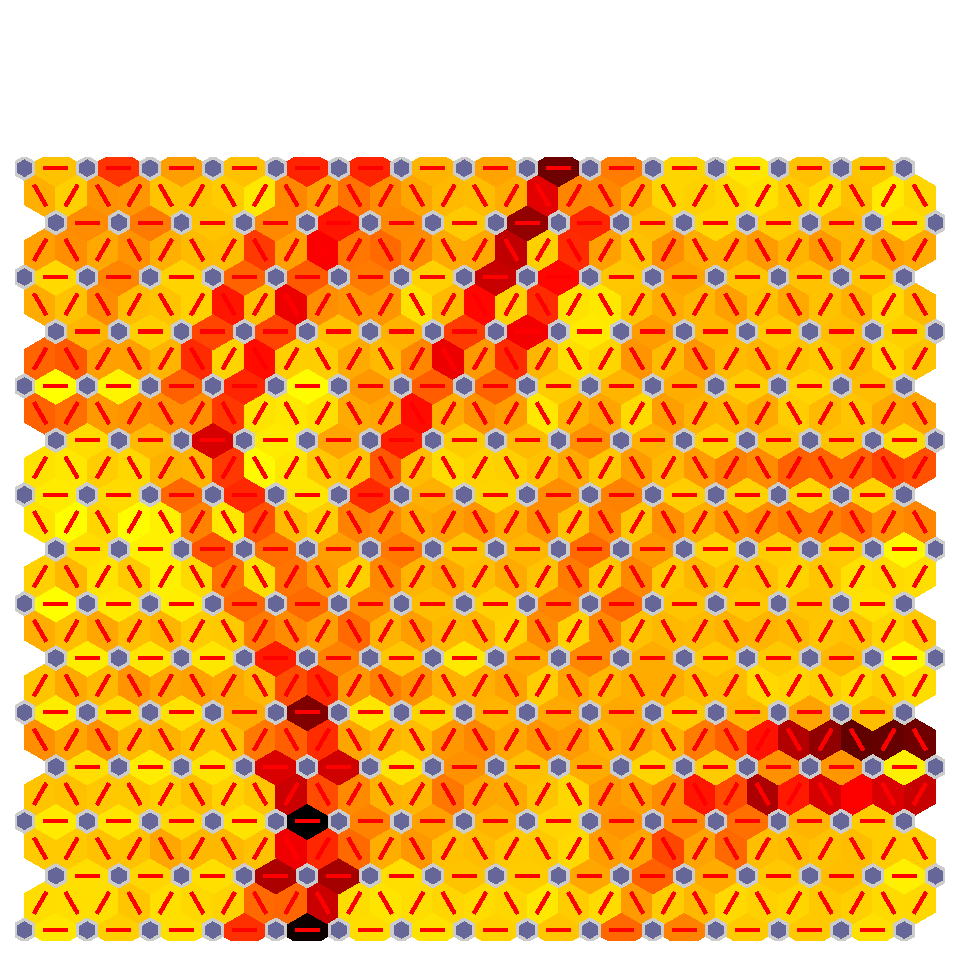
\includegraphics[width=\linewidth,keepaspectratio]{fashion_mnist_p2_u_matrix.pdf}\\{\small (b) Fashion-MNIST}
\end{minipage}
\caption{U-matrices of the $15\times15$ SOMs: distance between neighboring cells; high values mark borders between groups of cells. On Fashion-MNIST the strongest borders surround the footwear, while the clothing part has weak borders.}
\label{fig:umatrix}
\end{figure}

\subsubsection{Embedding length explains much of the SVHN result}
SVHN embeddings have a much smaller norm (mean length 5.8 against 40.3 on MNIST, and 8.5 against 20.7 on Fashion-MNIST). That out-of-distribution inputs tend to have smaller feature norms is a known effect~\cite{park2023featurenorm,yu2023blockselection,haas2024l2norm,liu2025neuralcollapse}. On MNIST, QE is strongly correlated with length (Spearman $-0.83$), which favors it; on Fashion-MNIST the correlation is weak ($-0.29$), while length alone separates SVHN almost perfectly (0.995). When the comparison is restricted to images whose embedding length lies within the 5th to 95th percentile of the Fashion-MNIST training lengths (9,478 Fashion-MNIST and 532 SVHN images), QE separates SVHN from Fashion-MNIST with an AUROC of 0.958 (95\% interval 0.953 to 0.962), far above the 0.789 of the full comparison. This suggests that the length difference accounts for much of the weak overall result. The 532 SVHN images in the band are atypical for SVHN, and the other detectors were not scored on this subset, so it does not show that QE beats them there. On MNIST only 8 SVHN images fall in the matching band, so no length-matched comparison is possible. This analysis is exploratory. Finally, SVHN images collapse onto one cell of the digit 4 on MNIST (86.5\% of them) and onto cells whose majority class is Bag on Fashion-MNIST (91\%), where the map treats them as typical bags. Figure~\ref{fig:svhn} shows where the SVHN images fall on the MNIST and Fashion-MNIST maps.

\begin{figure}[htbp]
\centering
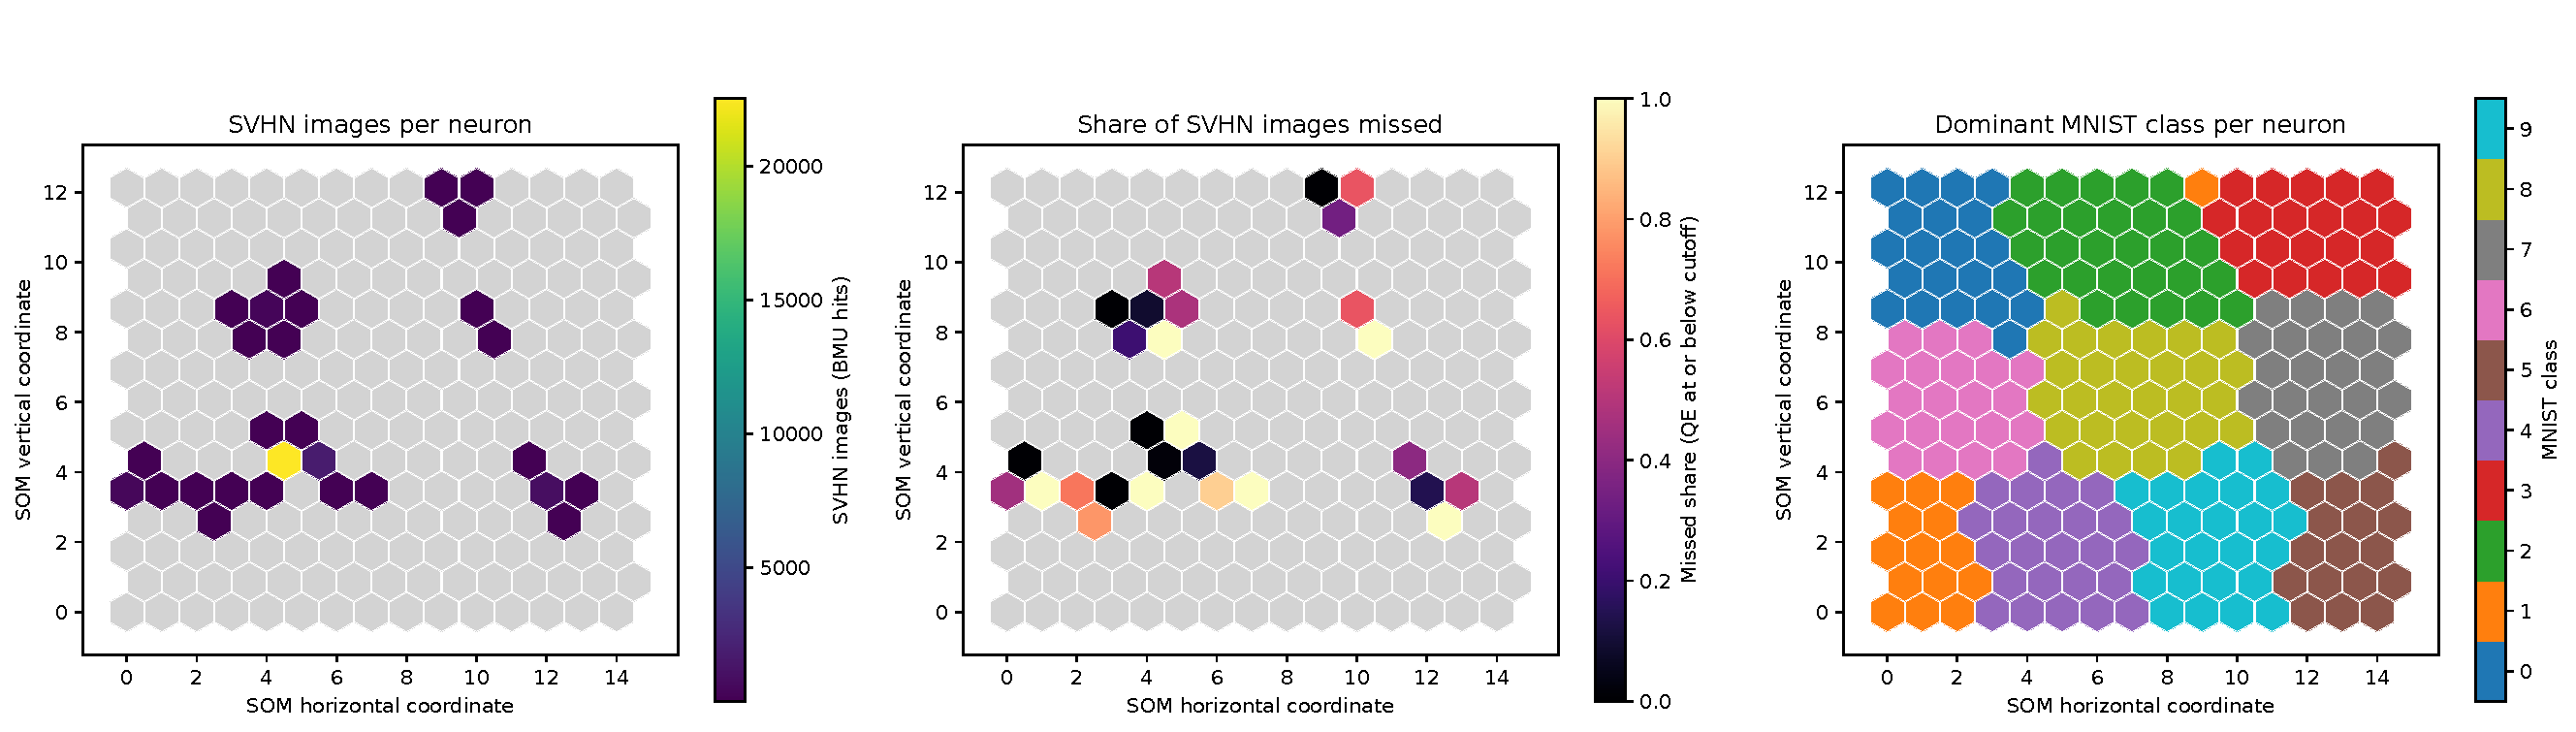
\includegraphics[width=\linewidth,height=0.3\textheight,keepaspectratio]{svhn_som_overlay_mnist.pdf}\\{\small (a) MNIST}\\[8pt]
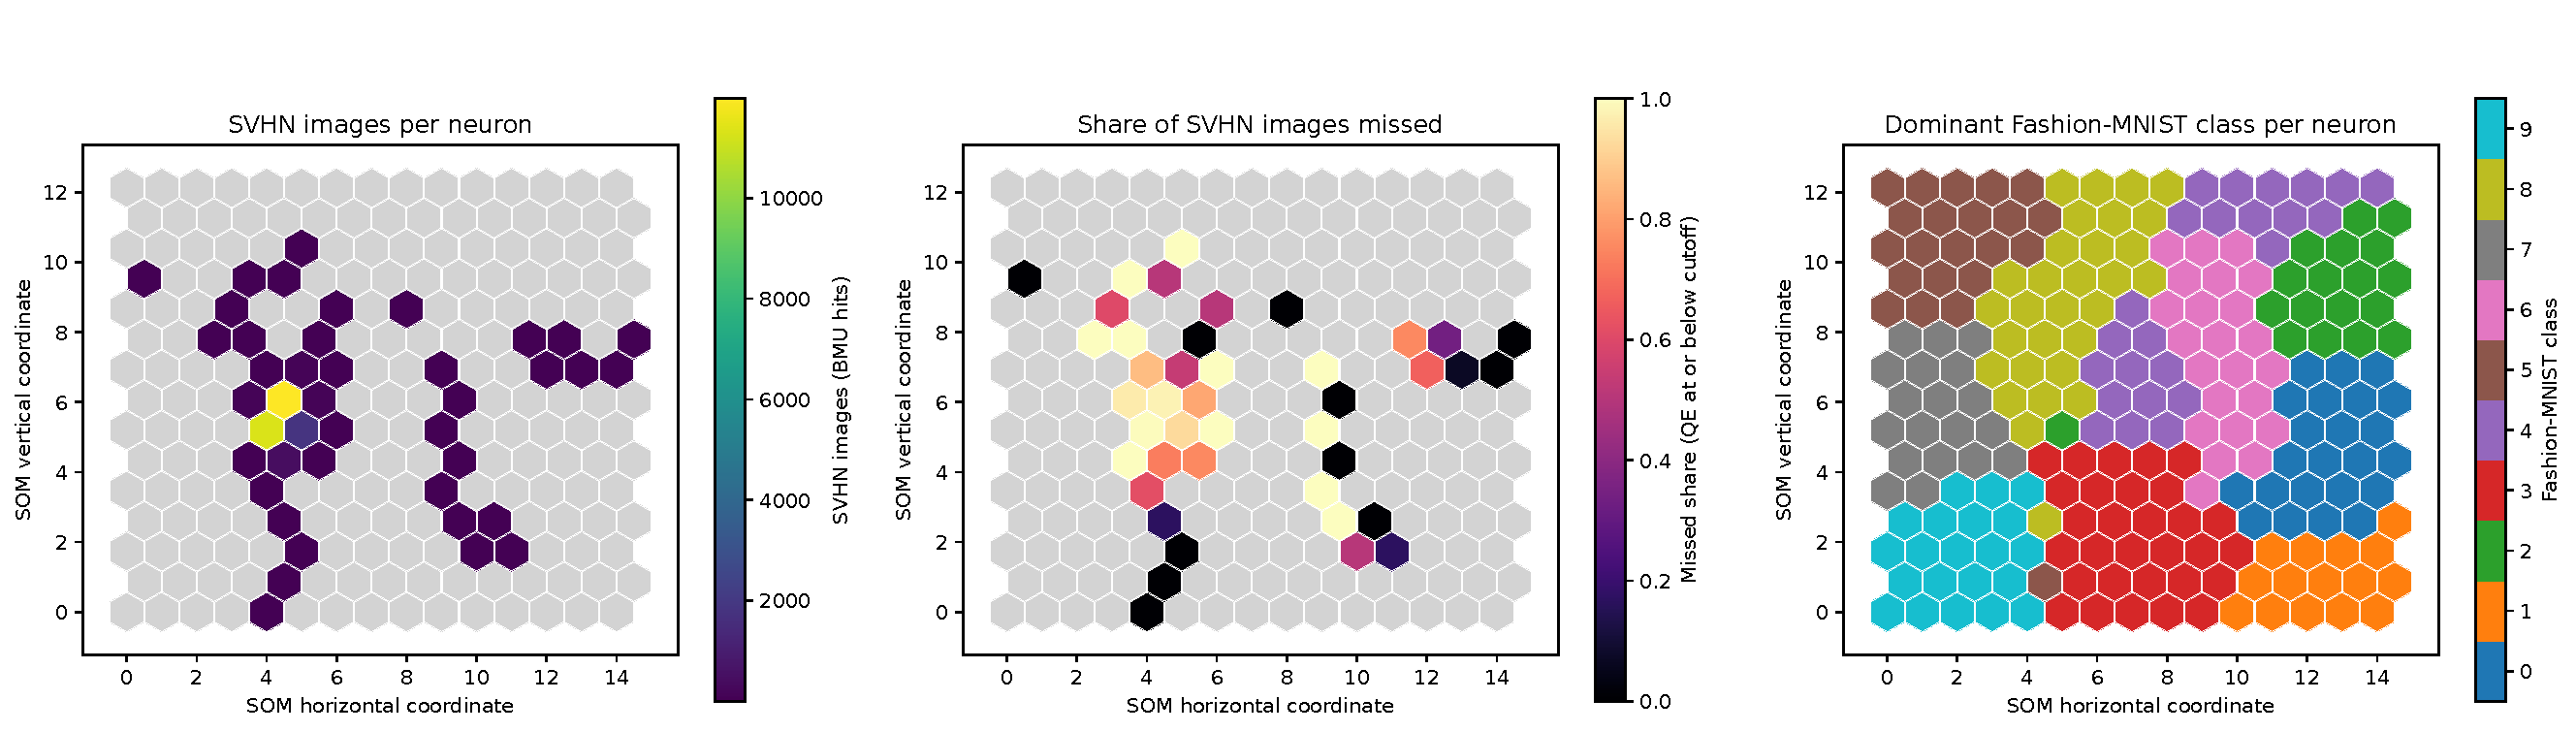
\includegraphics[width=\linewidth,height=0.3\textheight,keepaspectratio]{svhn_som_overlay_fashion_mnist.pdf}\\{\small (b) Fashion-MNIST}
\caption{SVHN images on the frozen $15\times15$ SOMs. In each row, left: number of SVHN images per cell; middle: share of the SVHN images in each cell that are missed, i.e.\ whose QE is at or below the training cutoff (1.569 for MNIST and 1.421 for Fashion-MNIST, the 95th percentile of the training QE); right: most common class of each cell (class numbers as in the dataset; on MNIST the class is the digit, on Fashion-MNIST 8 is Bag). Gray cells received no SVHN image.}
\label{fig:svhn}
\end{figure}

\subsection{Where the SOM scores higher: unseen classes of a similar kind}

Table~\ref{tab:near} reports the open-set experiment. The SOM detects the unseen classes in every split on both datasets (H1 supported; AUROC 0.860 to 0.957 on MNIST and 0.739 to 0.831 on Fashion-MNIST, against 0.500 for label permutation), and embedding length alone does not explain it (length alone: AUROC 0.630 to 0.889 on MNIST and 0.634 to 0.814 on Fashion-MNIST). On Fashion-MNIST the SOM outperforms the maximum softmax probability in all five splits (H2 supported, $+0.046$, $+0.034$ to $+0.057$); on MNIST the comparison is inconclusive ($-0.032$, $-0.095$ to $+0.032$). H3 is supported on Fashion-MNIST for the maximum softmax probability and inconclusive otherwise. H4 is contradicted on both datasets: the nearest-neighbor distance outperforms QE in every split, which indicates that the 225 cells discard some information in the training embeddings.

\begin{table}[htbp]
\centering
\caption{Near novelty detection on held-out classes (mean area under the receiver operating characteristic curve, AUROC, over 5 class splits).}
\label{tab:near}
\small
\begin{tabular}{L{0.40\textwidth}C{0.24\textwidth}C{0.24\textwidth}}
\toprule
 & \textbf{MNIST} & \textbf{Fashion-MNIST} \\ \midrule
SOM quantization error & 0.912 & 0.794 \\
Maximum softmax probability & 0.944 & 0.749 \\
Energy & 0.927 & 0.783 \\
Mahalanobis distance & 0.927 & 0.823 \\
Nearest-neighbor distance & \textbf{0.966} & \textbf{0.842} \\
QE minus max-softmax (95\% interval) & $-0.032$ ($-0.095$, $+0.032$) & $+0.046$ ($+0.034$, $+0.057$) \\
QE minus nearest neighbor (95\% interval) & $-0.054$ ($-0.084$, $-0.024$) & $-0.048$ ($-0.071$, $-0.026$) \\ \bottomrule
\end{tabular}

\par\vspace{3pt}
{\footnotesize\raggedright Four classes were held out of training in each of 5 splits, with a new network and map per split. Hypotheses were fixed before the run; intervals are $t$-intervals over the 5 splits.\par}
\end{table}

\subsection{Guided retraining: mixed results}

\subsubsection{Setting}
The SOM hard pool contains 4,217 images (8.6\% of the training set) on MNIST and 19,997 (40.8\%) on Fashion-MNIST. The augmentation ranges that passed the pre-training check were rotation $10^\circ$, shift 1 pixel, zoom 0.9--1.1 and shear $8^\circ$ on MNIST, and $2.5^\circ$, 0.25 pixels, 0.975--1.025 and $2^\circ$ on Fashion-MNIST; the first ranges failed the check on both datasets and were reduced by rules recorded in advance. The hotspot cells contain 146 test images on MNIST and 422 on Fashion-MNIST. The hotspots were chosen from validation errors, so the test set is the independent confirmation of the hotspot result. On the test images of the normally trained networks, the 11 hotspots hold 1.4\% of the images and about 18\% of the mistakes (about 12.8 times their share) on MNIST, and 4.0\% of the images and about 15\% of the mistakes (about 3.9 times) on Fashion-MNIST.

\begin{table}[htbp]
\centering
\caption{Test accuracy and hotspot error after retraining (mean of 5 seeds).}
\label{tab:retraining}
\small
\begin{tabular}{L{0.40\textwidth}C{0.1\textwidth}C{0.12\textwidth}C{0.1\textwidth}C{0.12\textwidth}}
\toprule
 & \multicolumn{2}{c}{\textbf{MNIST}} & \multicolumn{2}{c}{\textbf{Fashion-MNIST}} \\
\textbf{Arm} & \textbf{Accuracy} & \textbf{Hotspot error} & \textbf{Accuracy} & \textbf{Hotspot error} \\ \midrule
Normal training (CF1) & 99.11\% & 11.4\% & 90.66\% & 36.0\% \\
Augmentation, random images & 99.18\% & 10.3\% & 90.60\% & 35.0\% \\
Augmentation, least-confident images & 99.25\% & 8.5\% & 90.57\% & 35.2\% \\
Augmentation, SOM-chosen images (CF2) & 99.21\% & \textbf{7.8\%} & 90.62\% & 34.0\% \\
Curriculum, SOM order & 98.66\% & 21.4\% & 87.37\% & 51.8\% \\
Curriculum, random order & 99.07\% & 12.2\% & 89.15\% & 42.1\% \\
Curriculum, least-confident order (control) & 98.69\% & 22.6\% & 87.07\% & 50.0\% \\ \bottomrule
\end{tabular}

\par\vspace{3pt}
{\footnotesize\raggedright Hotspot error is measured on the test images in the 11 hotspot cells of the original map. The single Phase~1 networks scored 99.18\% and 90.90\%.\par}
\end{table}

\subsubsection{MNIST: the hotspot error falls, but the evidence is suggestive}
The hotspot error falls from 11.4\% to 7.8\% (a 31\% reduction; Table~\ref{tab:retraining}). The image-level interval for criterion A1 (SOM-chosen against random augmentation) excludes zero (Table~\ref{tab:criteria}), but it treats the five networks as one fixed sample. Computed from the five per-seed hotspot errors saved with the test results (an additional calculation, not a new experiment), the difference is $-2.47$ points with a 95\% $t$-interval of $-6.66$ to $+1.73$, which includes zero, whereas the difference from normal training stays clear ($-3.56$, $-5.92$ to $-1.20$). The benefit over random images is therefore suggestive, not established. The error outside the hotspots did not increase (A3 met).

\subsubsection{Fashion-MNIST: no significant improvement}
The hotspot error falls from 36.0\% to 34.0\% (a 6\% reduction), but no criterion is met. The hard pool covers 41\% of the training images and is therefore much less selective, and the augmentation ranges had to be four times smaller than on MNIST.

\subsubsection{The SOM is not a better selector than the network's confidence}
The difference in hotspot error between SOM-chosen and least-confident images (SOM minus least-confident) is $-0.7$ points ($-2.9$ to $+1.2$) on MNIST and $-1.2$ points ($-3.3$ to $+0.8$) on Fashion-MNIST. The two pools share 81\% of their images on Fashion-MNIST (16,213 of 19,997) and 47\% on MNIST (1,965 of 4,217), which is one reason why they behave alike. Using only the hotspot-cell images did not improve on normal training on either dataset ($-1.9$, $-4.4$ to $+0.7$ on MNIST; $+0.4$, $-1.8$ to $+2.5$ on Fashion-MNIST), and bringing the augmented images in gradually did not either; on MNIST the paced SOM arm was clearly worse than the unpaced one ($+3.4$ points, $+1.6$ to $+5.3$).

\begin{table}[htbp]
\centering
\caption{Phase 4 success criteria (fixed before the test; A1--A3 for augmentation, C1 and C2 for curriculum learning): difference in test error in percentage points, first arm minus second, with the 95\% paired bootstrap interval.}
\label{tab:criteria}
\small
\begin{tabular}{L{0.44\textwidth}C{0.24\textwidth}C{0.24\textwidth}}
\toprule
\textbf{Criterion} & \textbf{MNIST} & \textbf{Fashion-MNIST} \\ \midrule
A1 (primary): SOM copies beat random copies on hotspot error & $-2.47$ ($-4.52$, $-0.68$): met & $-1.04$ ($-3.22$, $+1.14$): not met \\
A2: SOM copies beat normal training on hotspot error & $-3.56$ ($-5.75$, $-1.37$): met & $-1.99$ ($-4.79$, $+0.71$): not met \\
A3: no damage outside the hotspots (upper end $\le 0.2$) & $-0.05$ ($-0.13$, $+0.02$): met & $+0.13$ ($-0.12$, $+0.37$): not met \\
C1: SOM curriculum beats normal training & $+0.45$: worse & $+3.29$: worse \\
C2: SOM curriculum beats random curriculum on hotspots & $+9.18$: worse & $+9.76$: worse \\ \midrule
A1 recomputed over the 5 seeds ($t$-interval; not pre-specified) & $-2.47$ ($-6.66$, $+1.73$) & $-1.04$ ($-2.37$, $+0.28$) \\
A2 recomputed over the 5 seeds ($t$-interval; not pre-specified) & $-3.56$ ($-5.92$, $-1.20$) & $-1.99$ ($-4.42$, $+0.44$) \\ \bottomrule
\end{tabular}

\par\vspace{3pt}
{\footnotesize\raggedright C1, C2, A1 and A2 also require the macro-F1 guard to hold.\par}
\end{table}

\subsubsection{Curriculum learning}
Curriculum learning lowered accuracy on both datasets, more strongly on Fashion-MNIST (Tables~\ref{tab:retraining} and~\ref{tab:criteria}). The schedule never uses more than 40\% of the hard pool, so the hardest 60\% is never trained on; this corresponds to about 5\% of all training images on MNIST and about a quarter on Fashion-MNIST. There was no catastrophic forgetting: the largest drop in validation accuracy between consecutive epochs was at most 0.6 points (MNIST) and 0.9 points (Fashion-MNIST) in every arm.

\subsubsection{New maps after retraining}
Training a new SOM on each retrained network, SOM guidance changes the SVHN QE AUROC by $+0.008$ ($-0.014$ to $+0.030$, inconclusive) on MNIST and lowers it by 0.123 ($-0.151$ to $-0.094$) on Fashion-MNIST. The maximum softmax probability and energy remain better in every network on MNIST, and embedding length alone achieves 0.9998 to 0.9999. Figures~\ref{fig:reanalysis} and~\ref{fig:reanalysis_f} report the measures of the new SOMs for each seed. On MNIST, the hotspots of the SOM-guided arm contain fewer errors than after normal training in every seed; on Fashion-MNIST they do not, and the new maps are less pure.

% Each panel is a clipped region (viewport) of the original two-row figure, so the PDF itself is unchanged
\begin{figure}[p]
\centering
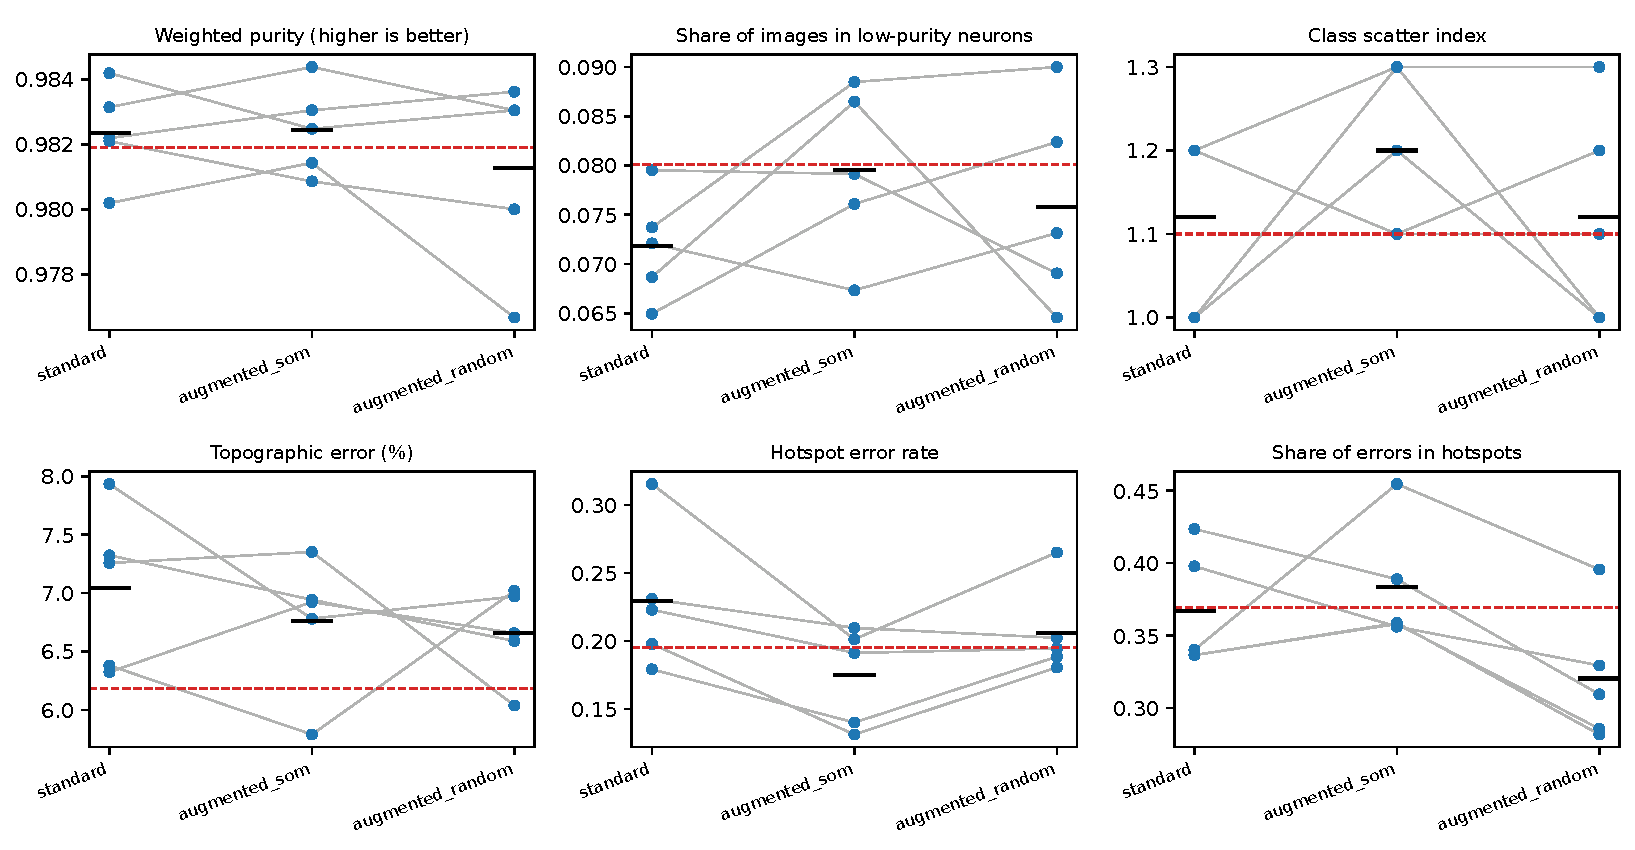
\includegraphics[viewport=0 204 264 402,clip,width=0.47\linewidth]{mnist_p4_map_measures_by_arm.pdf}\hfill
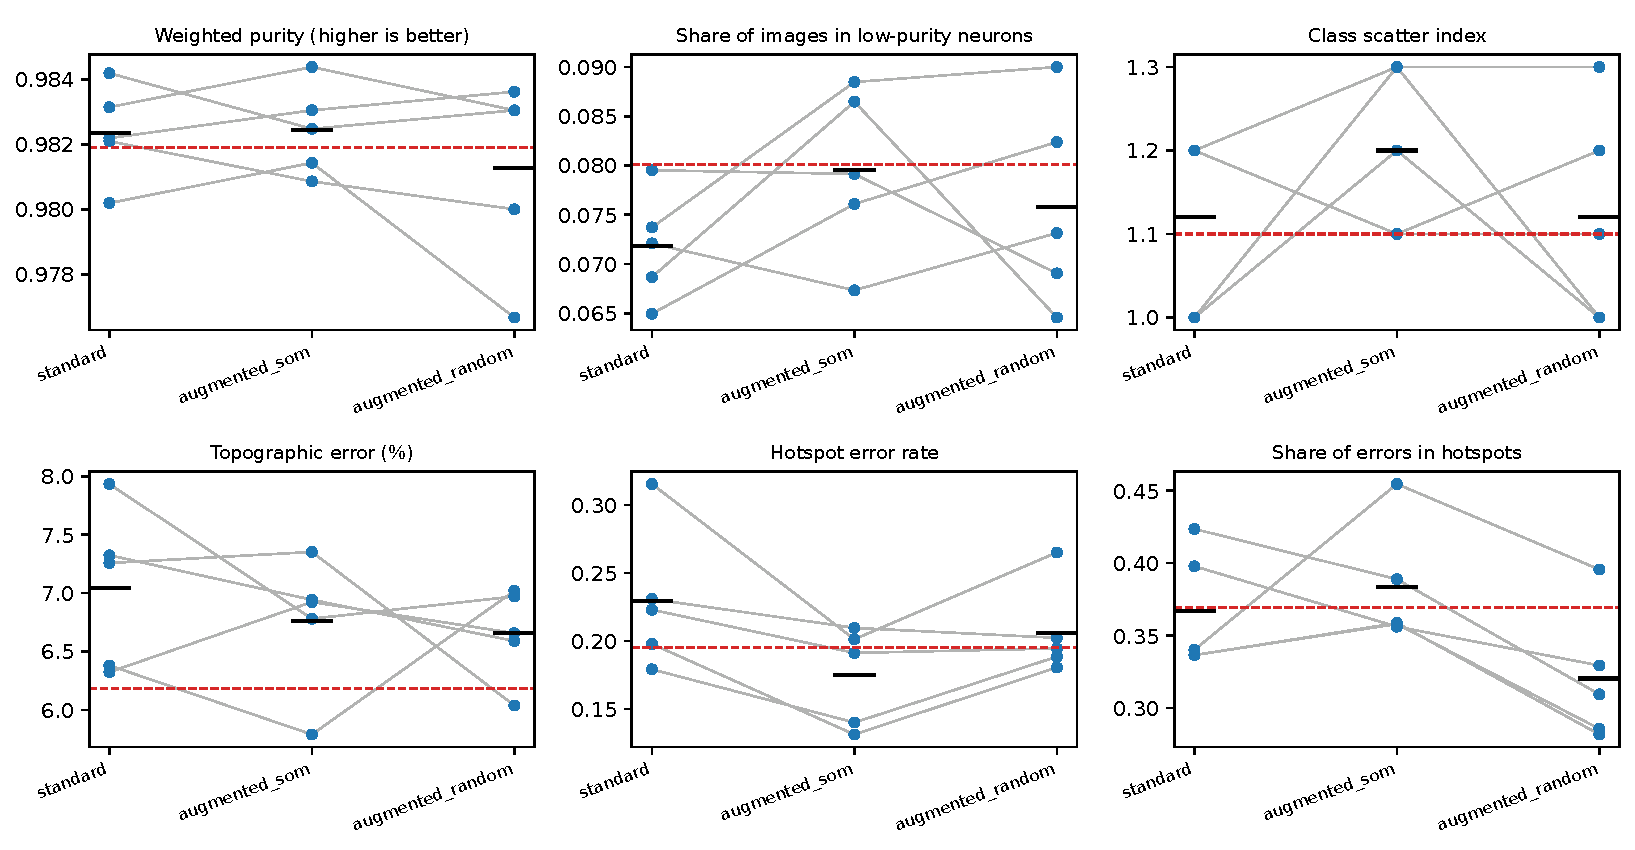
\includegraphics[viewport=264 204 522 402,clip,width=0.47\linewidth]{mnist_p4_map_measures_by_arm.pdf}\\[4pt]
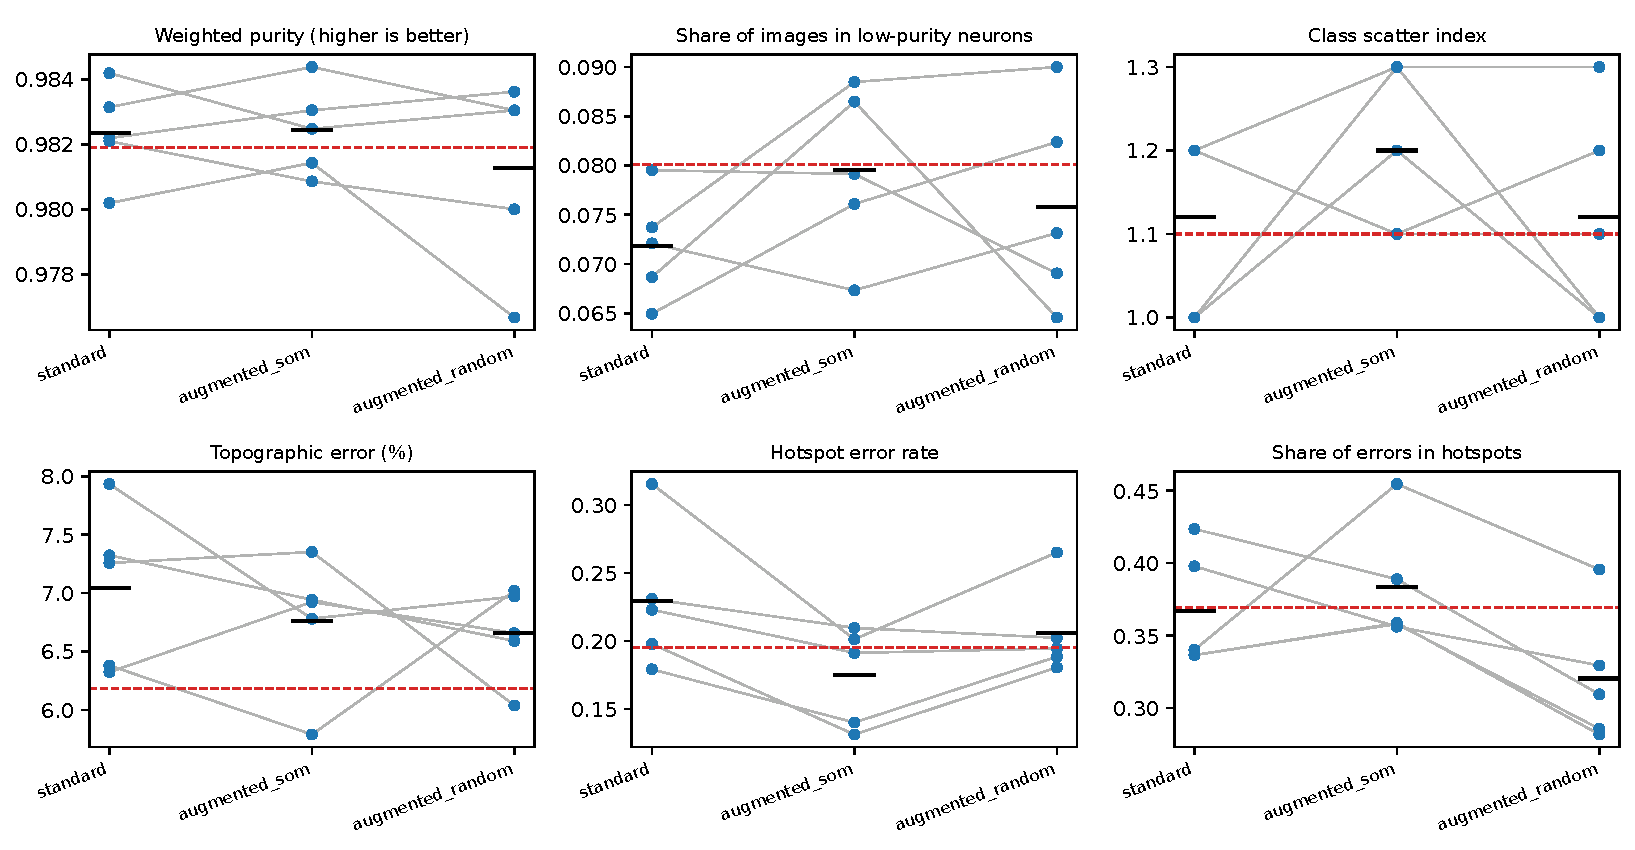
\includegraphics[viewport=522 204 785 402,clip,width=0.47\linewidth]{mnist_p4_map_measures_by_arm.pdf}\hfill
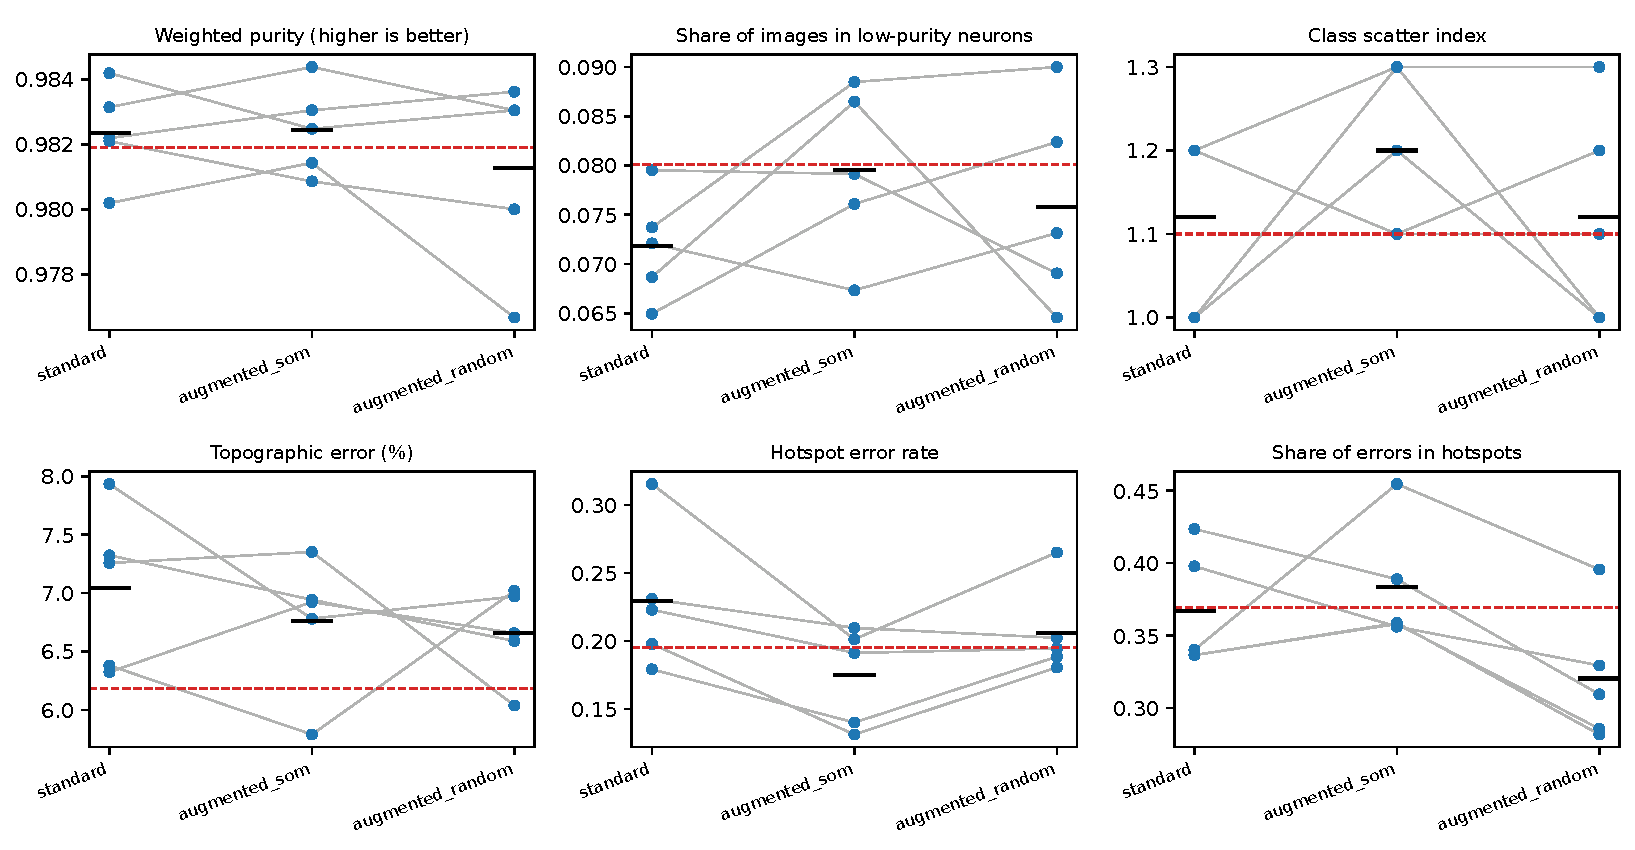
\includegraphics[viewport=0 2 264 202,clip,width=0.47\linewidth]{mnist_p4_map_measures_by_arm.pdf}\\[4pt]
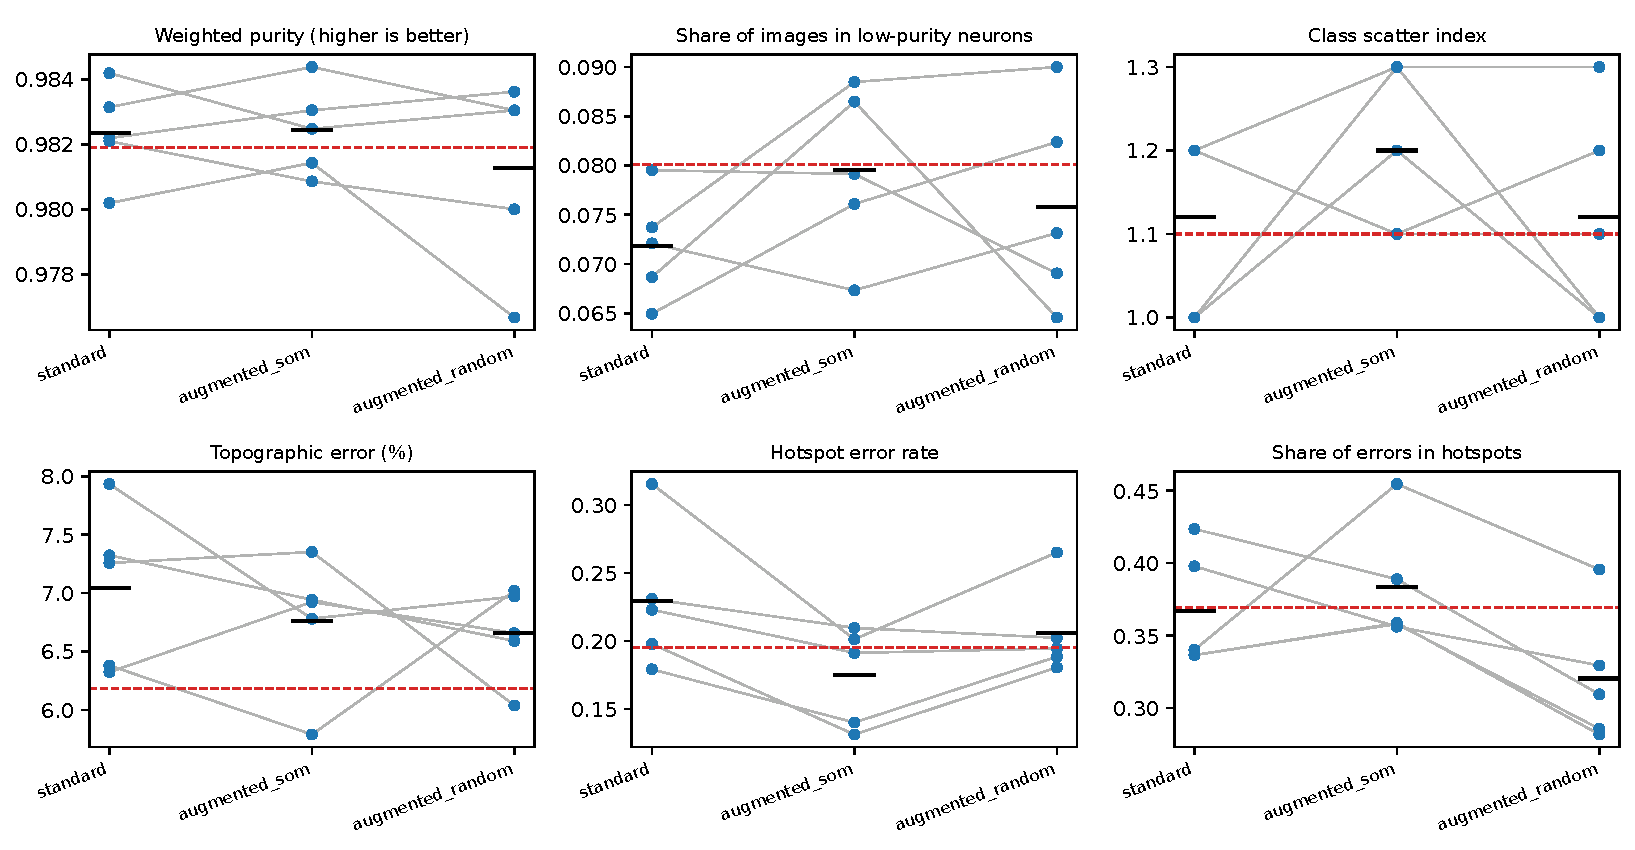
\includegraphics[viewport=264 2 522 202,clip,width=0.47\linewidth]{mnist_p4_map_measures_by_arm.pdf}\hfill
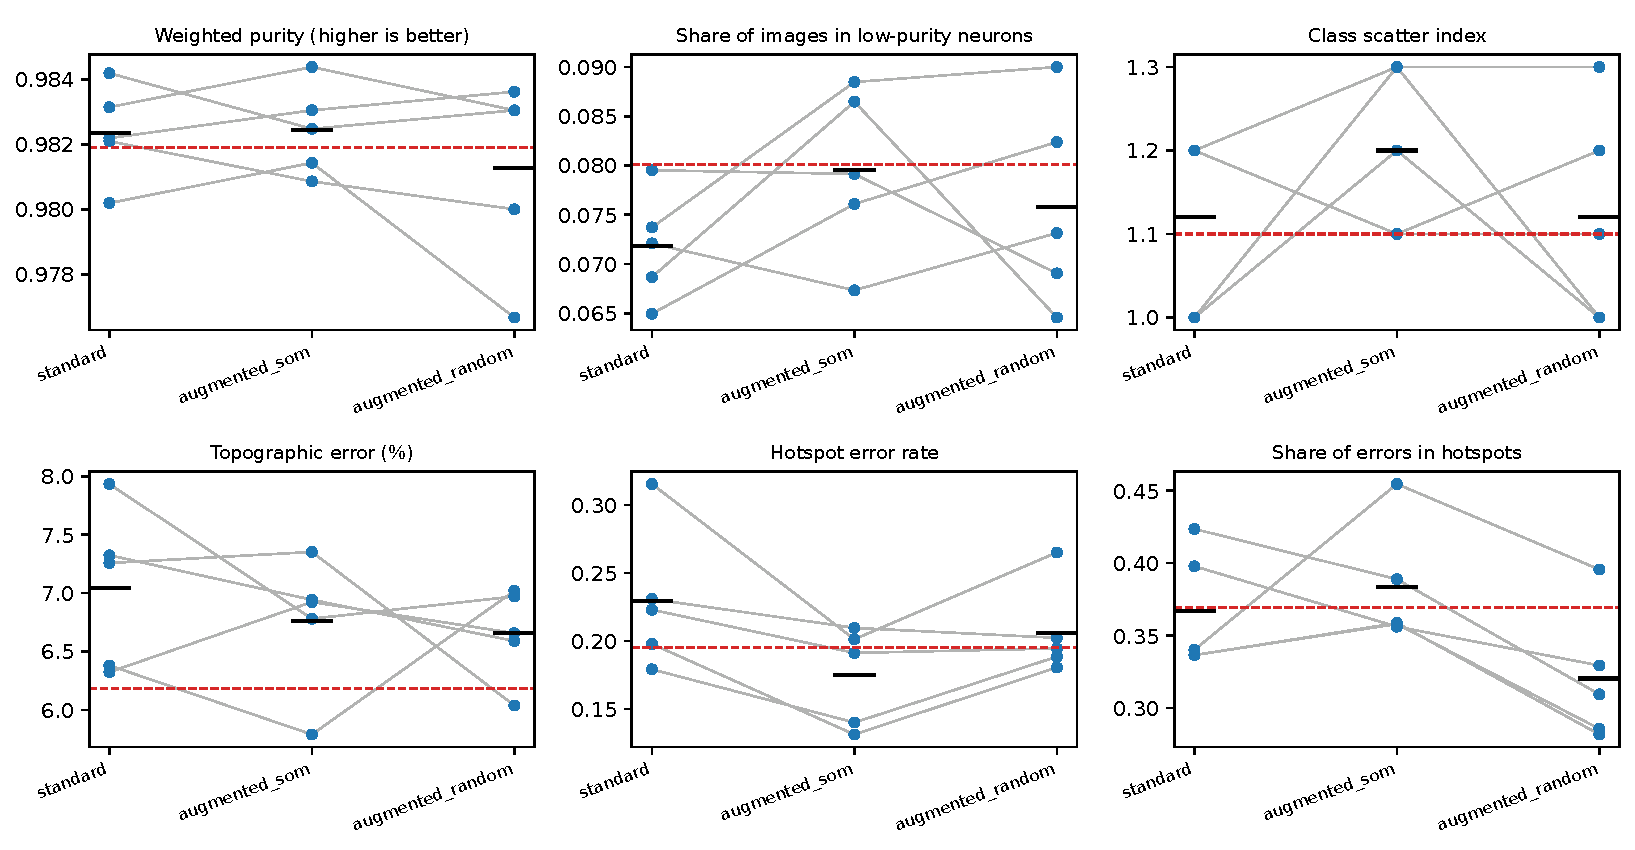
\includegraphics[viewport=522 2 785 202,clip,width=0.47\linewidth]{mnist_p4_map_measures_by_arm.pdf}
\caption{Measures of the new SOMs trained on the retrained MNIST networks, on validation images. Each dot is one CNN seed, the black bar is the mean over seeds, and the dashed line is the original (Phase~2) map. The arms are normal training (standard, CF1), SOM-guided augmentation (augmented\_som, CF2) and random augmentation (augmented\_random). The six panels are cut from one figure produced by the project code and enlarged for reading; their content is unchanged.}
\label{fig:reanalysis}
\end{figure}

\begin{figure}[p]
\centering
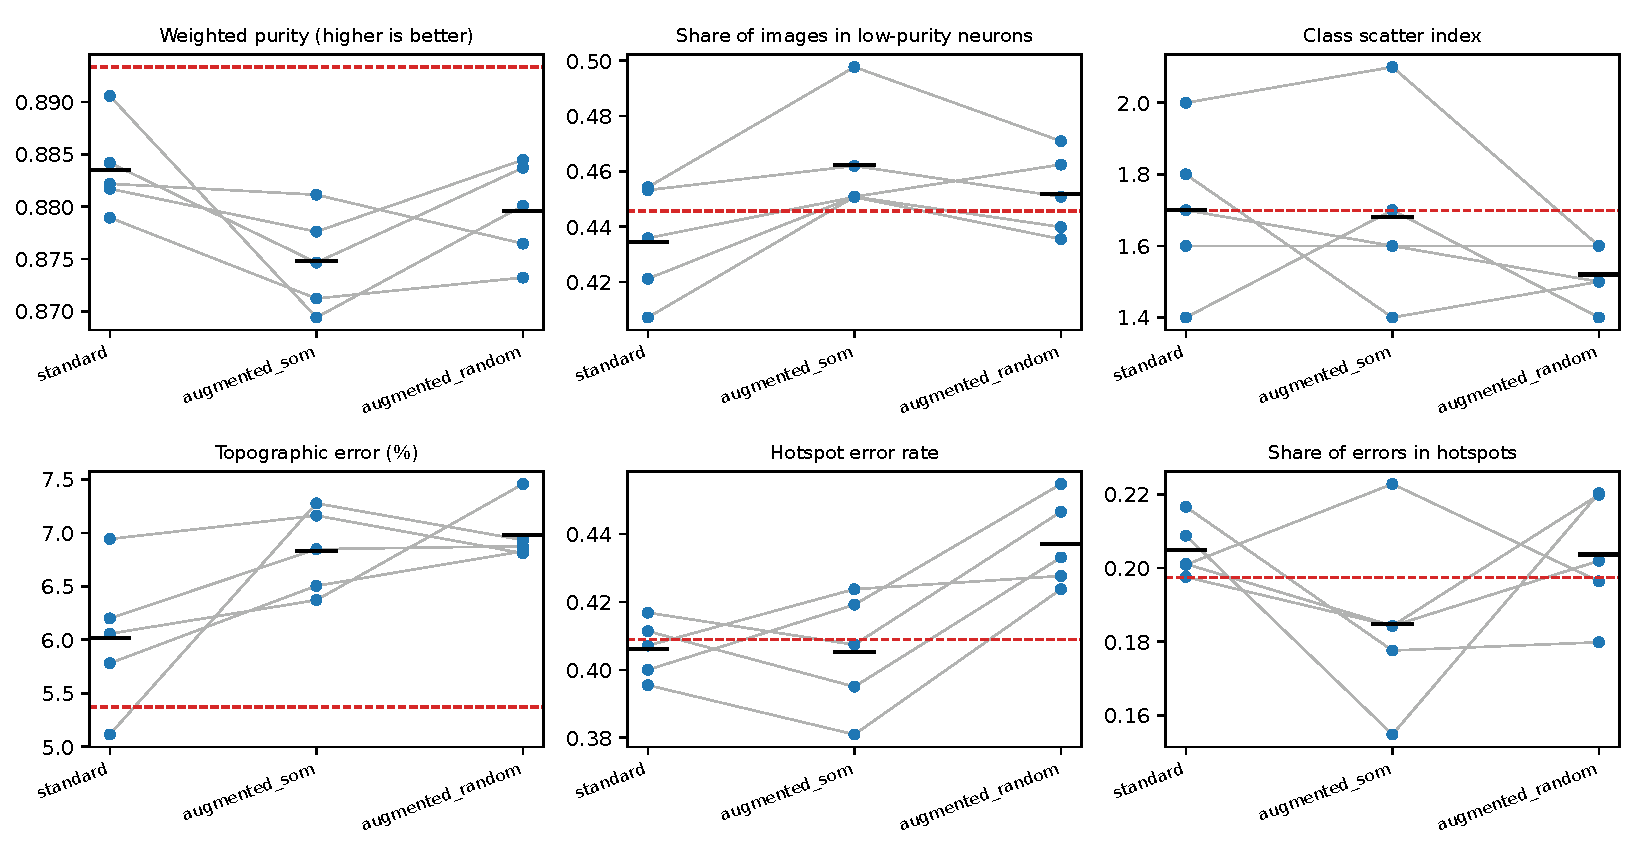
\includegraphics[viewport=0 204 264 402,clip,width=0.47\linewidth]{fashion_mnist_p4_map_measures_by_arm.pdf}\hfill
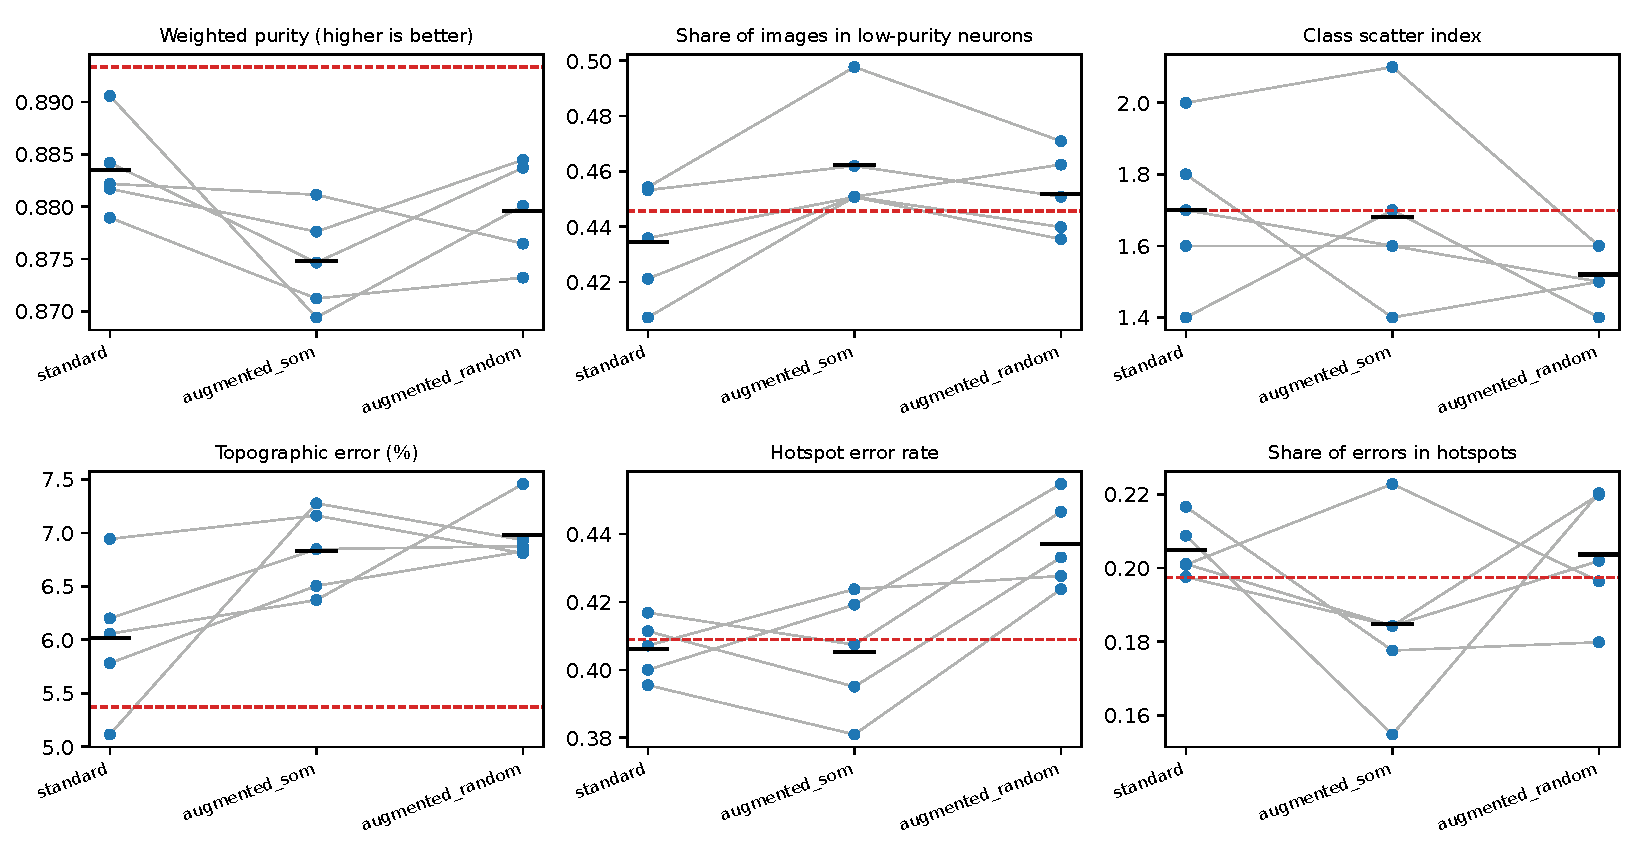
\includegraphics[viewport=264 204 522 402,clip,width=0.47\linewidth]{fashion_mnist_p4_map_measures_by_arm.pdf}\\[4pt]
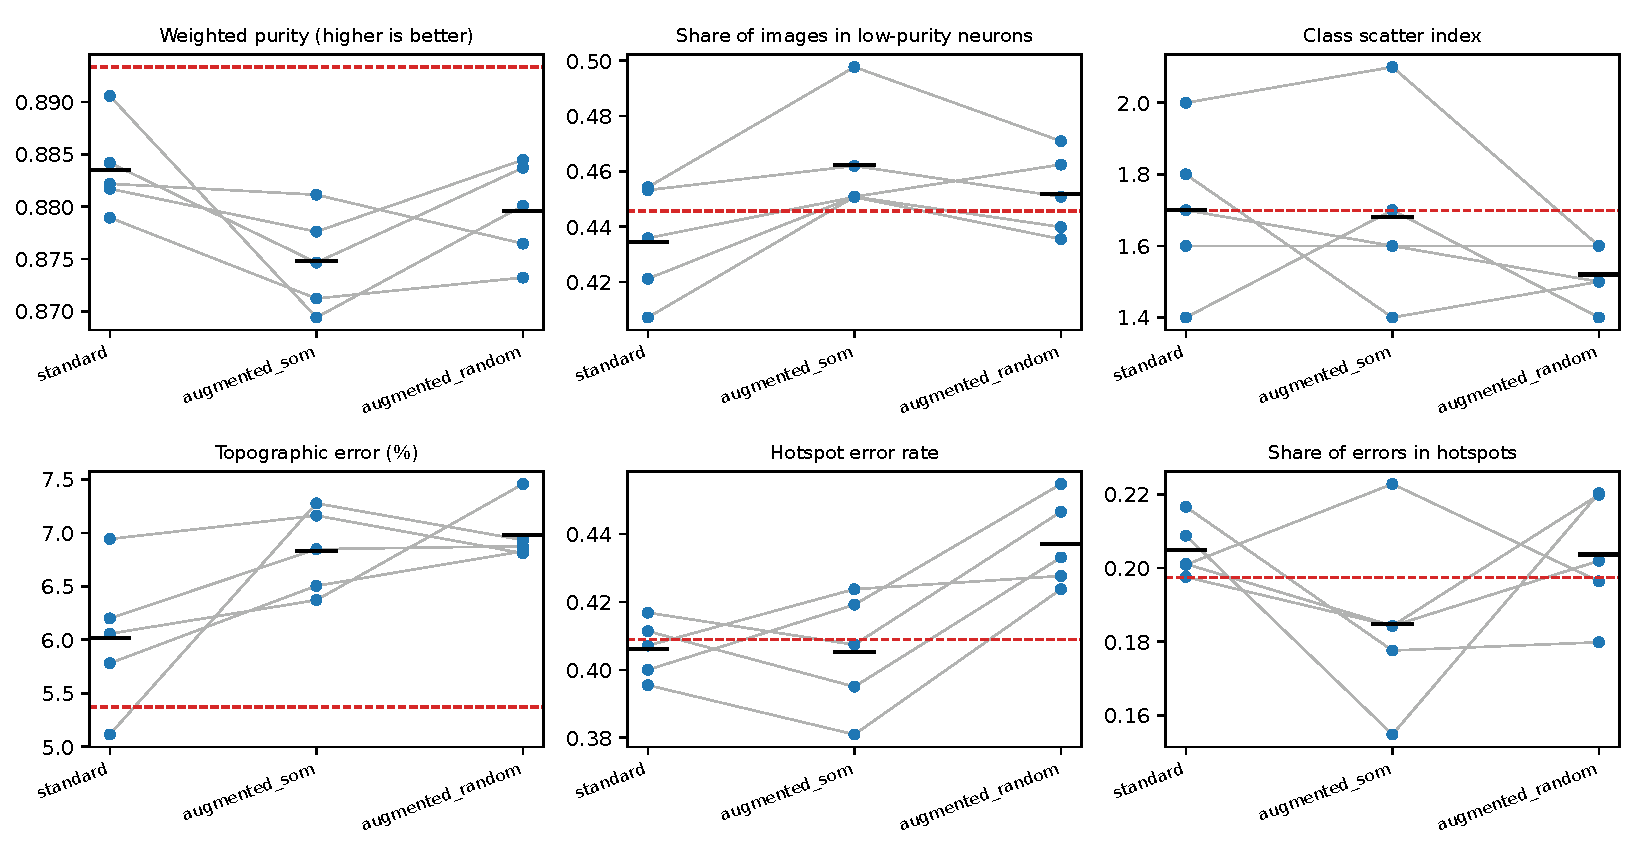
\includegraphics[viewport=522 204 785 402,clip,width=0.47\linewidth]{fashion_mnist_p4_map_measures_by_arm.pdf}\hfill
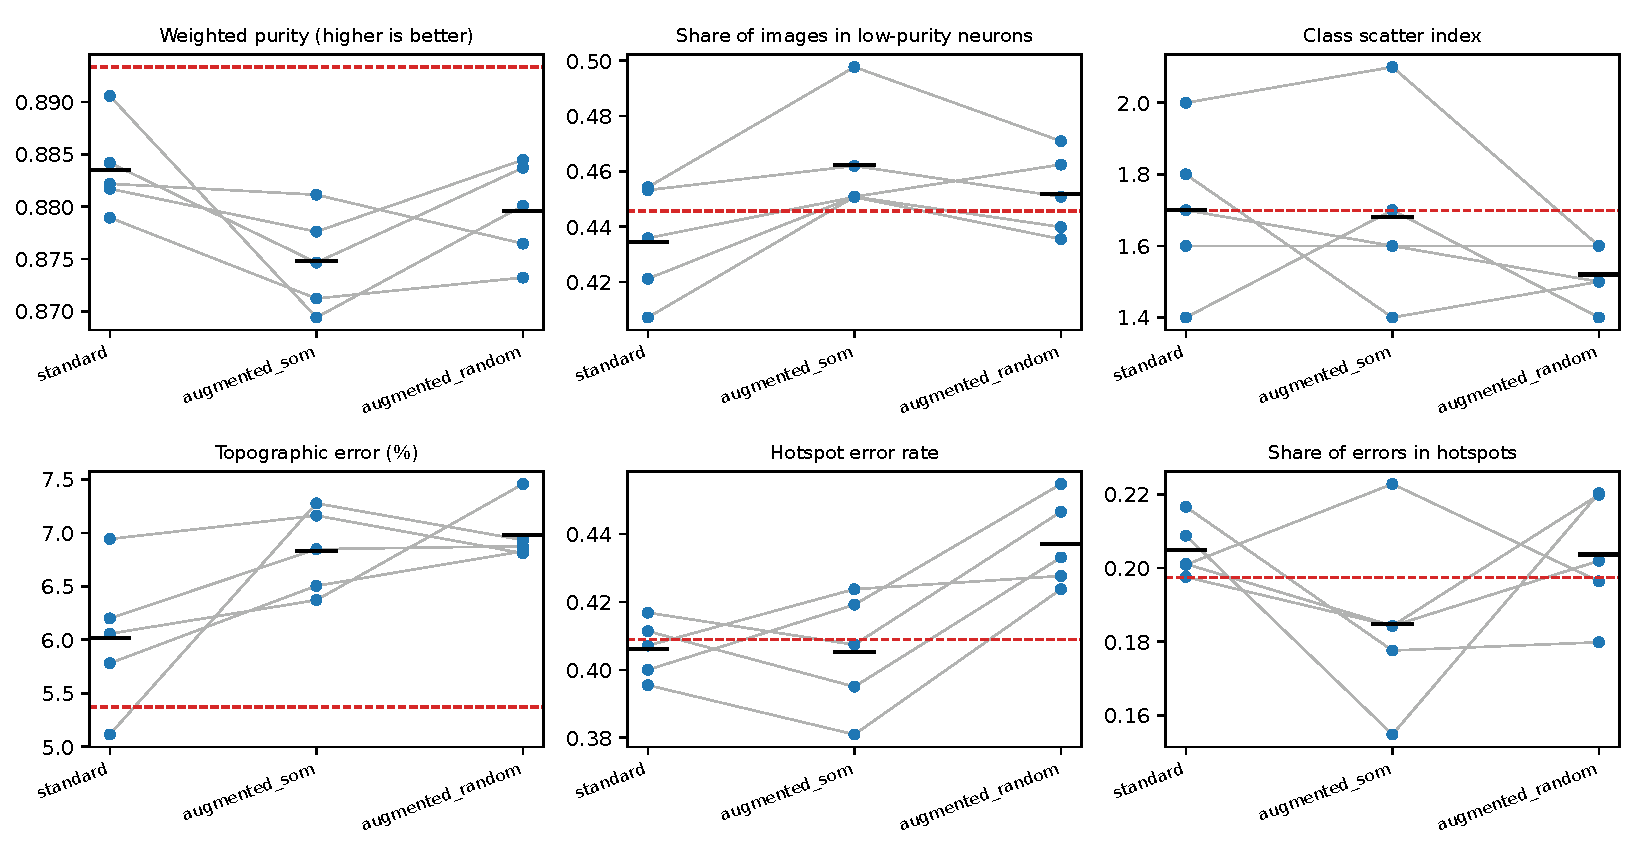
\includegraphics[viewport=0 2 264 202,clip,width=0.47\linewidth]{fashion_mnist_p4_map_measures_by_arm.pdf}\\[4pt]
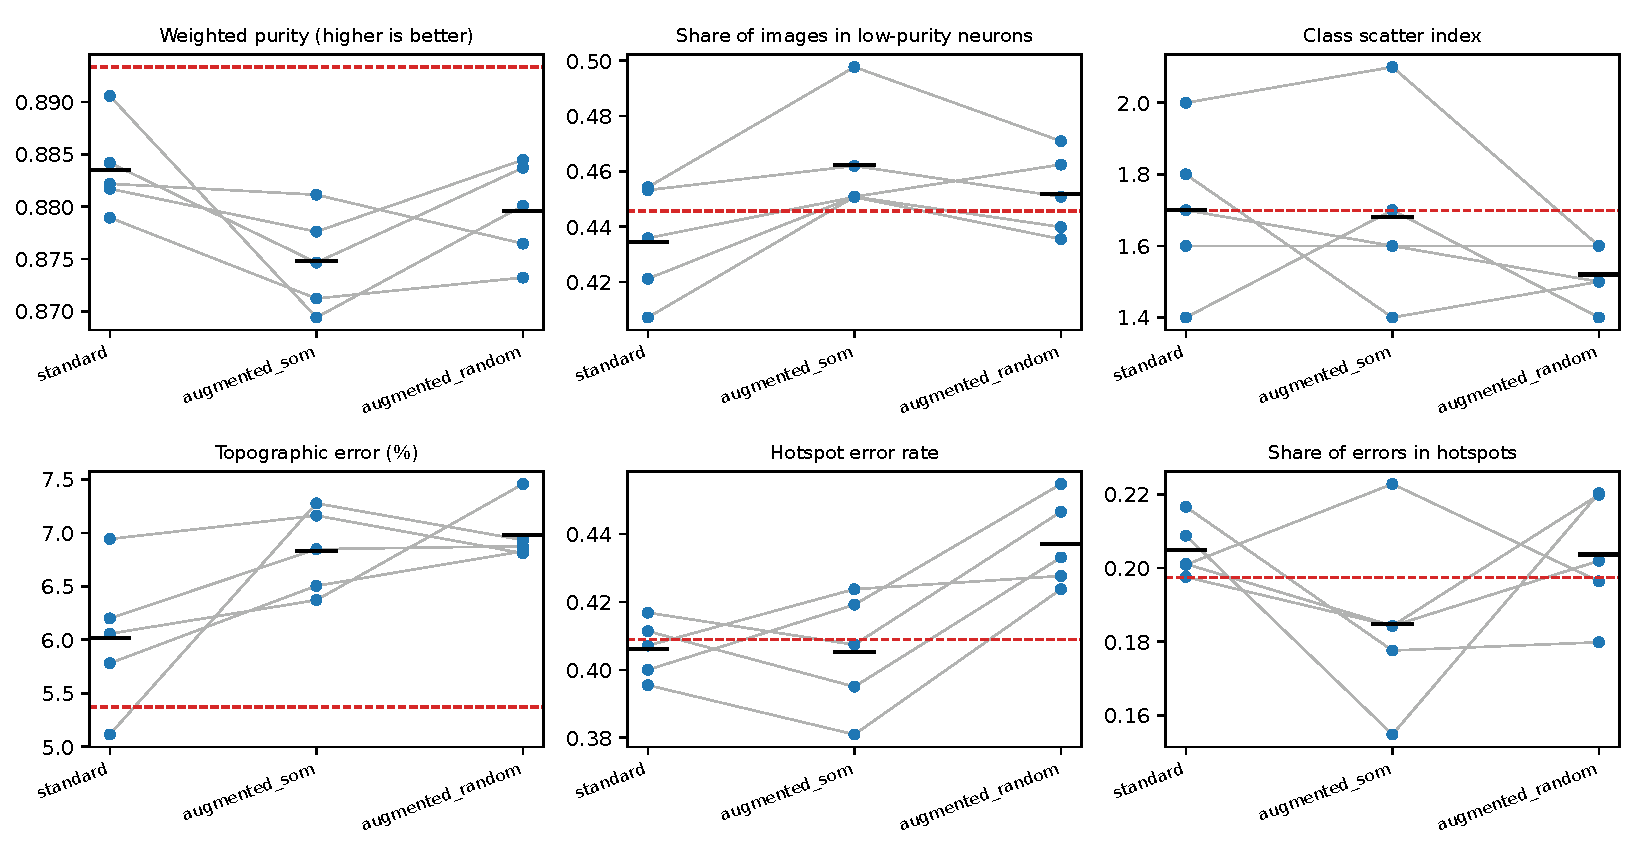
\includegraphics[viewport=264 2 522 202,clip,width=0.47\linewidth]{fashion_mnist_p4_map_measures_by_arm.pdf}\hfill
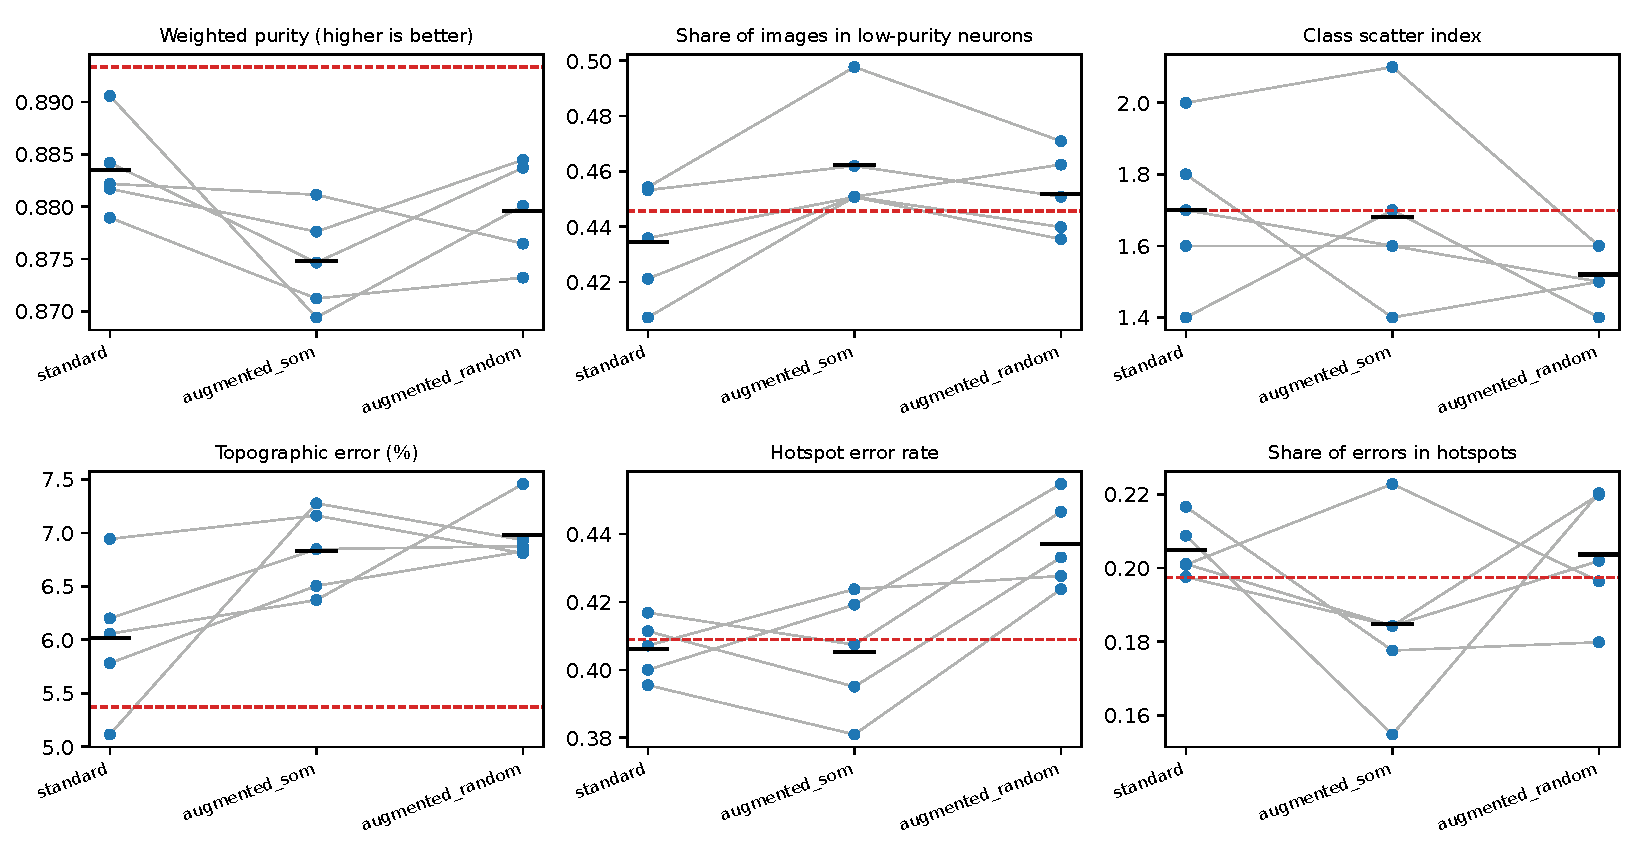
\includegraphics[viewport=522 2 785 202,clip,width=0.47\linewidth]{fashion_mnist_p4_map_measures_by_arm.pdf}
\caption{The same measures as in Fig.~\ref{fig:reanalysis}, for the new SOMs trained on the retrained Fashion-MNIST networks.}
\label{fig:reanalysis_f}
\end{figure}

\subsubsection{End-to-end comparison}
Table~\ref{tab:endtoend} compares CF1 with CF2 on the same 10,500 test images, and Fig.~\ref{fig:cf} shows the confusion matrices. On MNIST a few confusions become less frequent; on Fashion-MNIST the main change is an exchange of errors between Shirt and T-shirt/top. Per seed, CF2 fixed about 40 of the CF1 mistakes on MNIST and made about 30 new ones, so the net change over all images ranged from $-12$ to $+31$ mistakes; on Fashion-MNIST it fixed about 335 and made about 340 new ones ($-49$ to $+69$). In the hotspot cells the balance was better on MNIST (about 8 fixed and 3 new per seed) than on Fashion-MNIST (about 56 fixed and 47 new). The reduction is therefore real in the hotspot cells but is accompanied by mistakes elsewhere, and its size varies between seeds. The per-class error, which does not depend on the map, shows the same: on MNIST only the digit 9 changes significantly (1.30\% to 0.98\%, $-0.33$ points, $-0.67$ to $-0.04$), one of the digits of the dominant 4--9 confusion; on Fashion-MNIST the error of Shirt falls from 28.7\% to 26.4\% ($-2.3$ points, $-3.5$ to $-1.0$), whereas those of T-shirt/top (13.4\% to 14.8\%), Dress (7.5\% to 8.4\%) and Bag (1.7\% to 2.7\%) rise significantly.

\begin{table}[htbp]
\centering
\caption{End-to-end comparison of CF1 (normal training) and CF2 (SOM-guided retraining), mean over 5 seeds.}
\label{tab:endtoend}
\small
\begin{tabular}{L{0.50\textwidth}C{0.20\textwidth}C{0.20\textwidth}}
\toprule
\textbf{Measure} & \textbf{MNIST} & \textbf{Fashion-MNIST} \\ \midrule
Test mistakes, CF1 / CF2 & 93.2 / 82.6 & 980.6 / 985.2 \\
Hotspot mistakes, CF1 / CF2 & 16.6 / 11.4 & 151.8 / 143.4 \\
Seeds with fewer hotspot mistakes in CF2 & 5 of 5 & 4 of 5 \\
Mistakes fixed / new mistakes per seed & about 40 / 30 & about 335 / 340 \\
Net change over all images (fixed minus new; positive = CF2 better), range over seeds & $-12$ to $+31$ & $-49$ to $+69$ \\ \bottomrule
\end{tabular}

\par\vspace{3pt}
{\footnotesize\raggedright A mistake is \emph{fixed} if CF1 is wrong and CF2 is right on that image, and \emph{new} if CF1 is right and CF2 is wrong. The net change is the number of mistakes of CF1 minus those of CF2: a positive value means CF2 made fewer mistakes, a negative value means it made more.\par}
\end{table}

\begin{figure}[htbp]
\centering
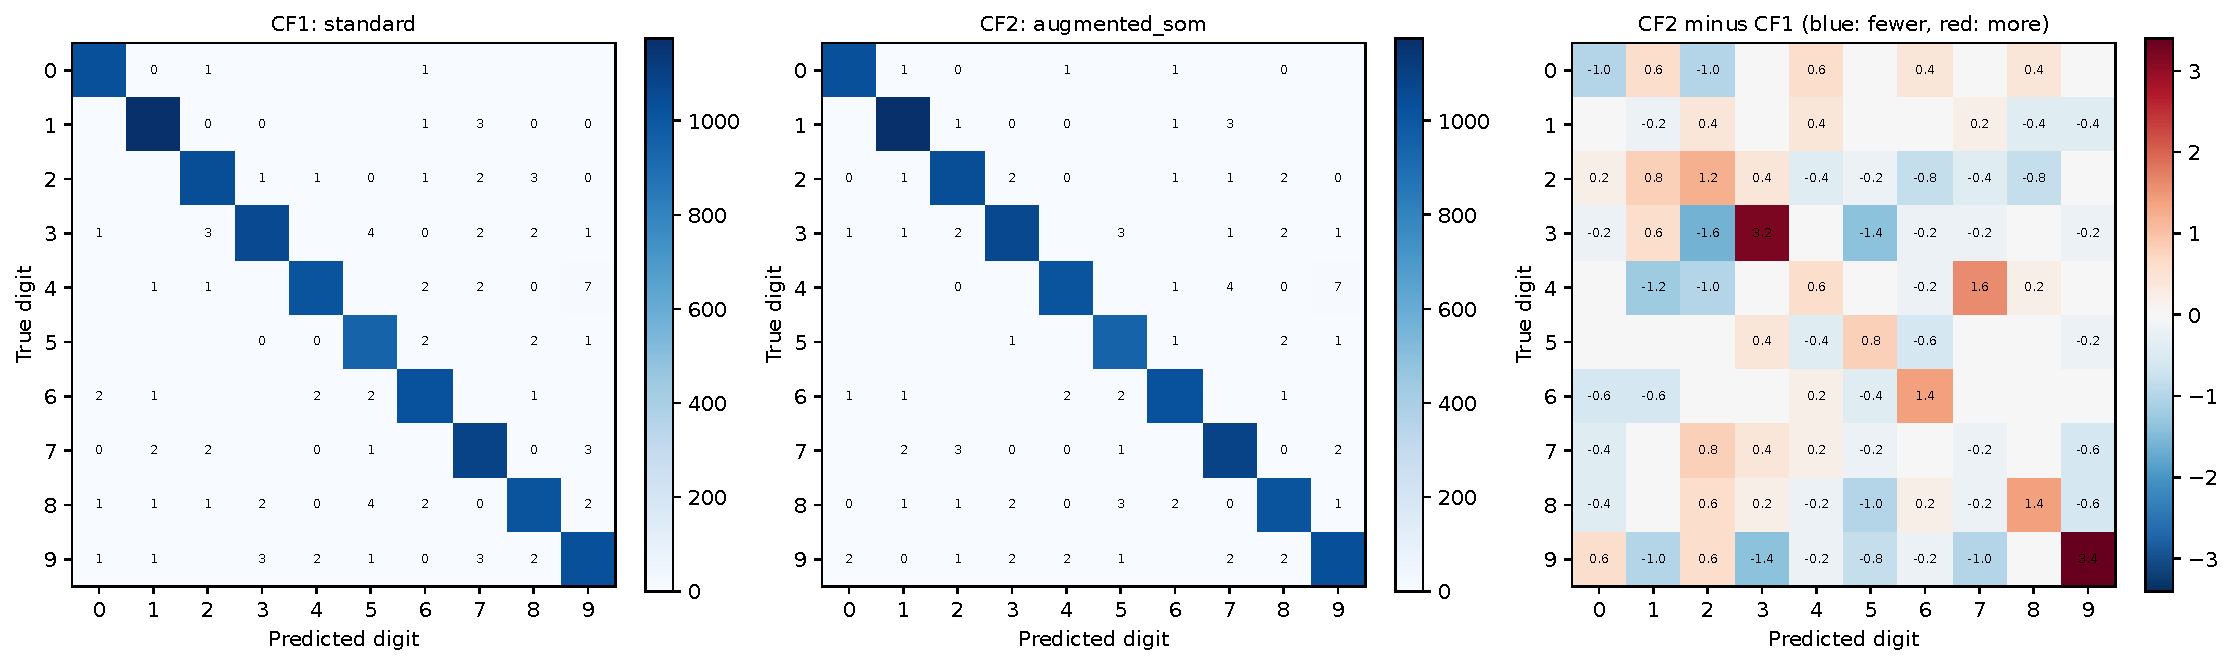
\includegraphics[width=\linewidth,height=0.3\textheight,keepaspectratio]{mnist_p4_confusion_standard_vs_augmented_som.pdf}\\{\small (a) MNIST}\\[8pt]
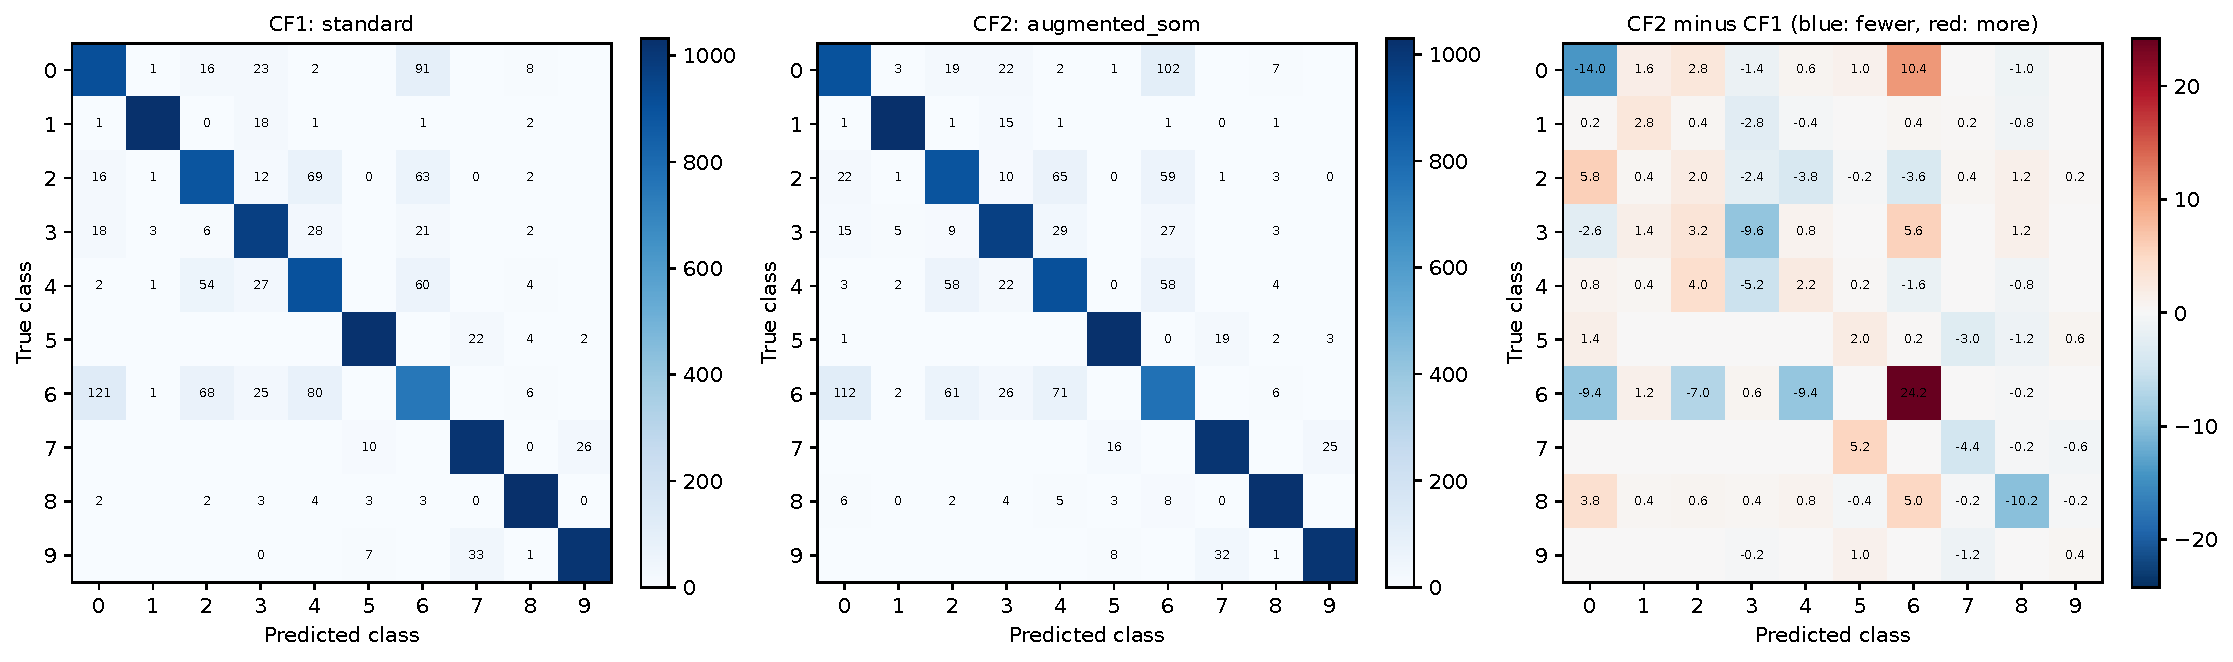
\includegraphics[width=\linewidth,height=0.3\textheight,keepaspectratio]{fashion_mnist_p4_confusion_standard_vs_augmented_som.pdf}\\{\small (b) Fashion-MNIST}
\caption{Mean test confusion matrices over 5 seeds for CF1 (normal training; panel title ``standard'') and CF2 (SOM-guided augmentation; panel title ``augmented\_som''), and their difference CF2 minus CF1 (blue: fewer cases, red: more cases). Rows are true classes and columns are predicted classes.}
\label{fig:cf}
\end{figure}

\subsection{Summary}

\begin{table}[htbp]
\centering
\caption{What works, what does not, and what works best.}
\label{tab:summary}
\footnotesize
\begin{tabular}{L{0.22\textwidth}L{0.42\textwidth}L{0.28\textwidth}}
\toprule
\textbf{Task} & \textbf{SOM result} & \textbf{What works best} \\ \midrule
Class structure and error location & Works: purity 98.2\% / 89.3\%; errors 11.1 / 3.9 times their share in 11 cells & The map itself (no scalar score gives this view) \\
Error detection & Does not beat simpler methods: AUROC 0.685 / 0.811, k-means 0.693 / 0.812 & Network confidence (0.981 / 0.906) \\
Far novelty (SVHN) & Detects it, but weaker: QE 0.981 / 0.789 & Energy score (0.9998 / 0.982) \\
Near novelty (unseen classes) & Higher than max-softmax on Fashion-MNIST (+0.046); inconclusive on MNIST & Nearest-neighbor distance (0.966 / 0.842) \\
Guided retraining & MNIST hotspot error 11.4\% $\rightarrow$ 7.8\% (suggestive at seed level); not significant on Fashion-MNIST & Least-confident selection (not significantly different) \\
Curriculum learning & Does not work: accuracy lowered on both datasets & Plain training \\ \bottomrule
\end{tabular}

\par\vspace{3pt}
{\footnotesize\raggedright Values are MNIST / Fashion-MNIST.\par}
\end{table}

% ------------------------------------------------------------------------------------------------------------------------
\FloatBarrier
\section{Discussion}\label{sec:discussion}

\subsection{The contribution of the SOM is the map, not the score}
As a scoring method, the SOM does not outperform the strongest simple baselines on either dataset (Table~\ref{tab:summary}). We therefore do not present it as a better detector. Its contribution is the map itself: a single, topology-preserving view of the feature space that shows where errors concentrate, which classes overlap, and where novel inputs are placed, information that a scalar score does not convey. Figures~\ref{fig:errormaps} and~\ref{fig:errormaps_f} show this most directly: the cells with many mistakes lie where two classes meet, which is also where the hard-example pool for retraining is drawn from.

\subsection{Why the results look the way they do}
The following explanations are consistent with our results, but we did not test them as causes.
\begin{itemize}
  \item \emph{Errors concentrate where classes overlap.} The error rate of a cell is strongly related to its class mixture (Spearman $-0.81$ and $-0.95$), and on Fashion-MNIST most hotspots mix upper-body garments whose distinguishing details occupy only a few pixels.
  \item \emph{K-means matches the SOM in AUROC.} Both quantize the same 84-dimensional embeddings into 225 prototypes and score a cell by its error rate, so they carry similar information; the network's confidence uses the classifier's own decision geometry, which the embedding-only maps do not see.
  \item \emph{QE is weak for SVHN on Fashion-MNIST.} SVHN embeddings are much shorter than the in-distribution ones, and the QE correlates with length on MNIST but not on Fashion-MNIST. On the 532 SVHN images of ordinary length, QE separates SVHN well (AUROC 0.958); the other detectors were not scored on that subset.
  \item \emph{The SOM scores higher than confidence on unseen clothing classes.} The network often assigns an unseen garment to a similar known class with high confidence, while the map still places it away from the known prototypes.
  \item \emph{Guided retraining helps less on Fashion-MNIST.} The hard pool covers 41\% of the training images, so it is far less selective, the augmentation ranges had to be four times smaller, and the SOM pool shares 81\% of its images with the least-confident pool.
  \item \emph{Curriculum learning hurts.} The schedule never trains on the hardest 60\% of the pool.
\end{itemize}

\subsection{What the SOM reveals beyond standard metrics}
Accuracy and the confusion matrix indicate how many errors occur and between which classes. The map additionally shows that the errors lie in regions where classes overlap and how large these regions are: a few small cells with atypical handwriting on MNIST, and one broad region of upper-body garments on Fashion-MNIST. It also shows how novel inputs are represented, which helps explain why a fixed QE threshold works on one dataset and fails on the other.

\subsection{Limitations}
\begin{itemize}
  \item LeNet-5 is the only CNN studied, and only two $28\times28$ grayscale datasets were used. The findings describe how the SOM behaves on the features of this small network; we did not test deeper architectures such as residual networks (ResNet).
  \item The headline Phase 2 and Phase 3 results use one network and one SOM seed; with the SOM seed alone, the Fashion-MNIST SVHN AUROC ranges from 0.766 to 0.884 over 5 SOM seeds. MNIST yields only 92 validation errors, so differences smaller than about 0.1 AUROC cannot be detected.
  \item SVHN is the only out-of-distribution dataset and it differs mainly in embedding length, also after retraining. The near-novelty splits share images and classes, so their $t$-intervals may be too narrow, and the random draw left the classes unbalanced.
  \item The baseline comparison covers only the $15\times15$ map, and on MNIST it uses three k-means initializations per seed. The headline grid was adopted by project decision, not by the selection rule (Section~\ref{sec:method}).
  \item In Phase 4 the hotspots are defined by the SOM, which favors the SOM-guided arms on hotspot error; the pools come from a single SOM; and five seeds can only resolve relatively large differences. All Fashion-MNIST settings were copied from MNIST by design, so the pool rule and the curriculum schedule were not adapted to a dataset with many more errors.
  \item The proposal asked for aggressive augmentation of high-error regions. The pre-training check limited the ranges, and on Fashion-MNIST the baseline network classified altered hotspot images almost as well as the originals (58.4\% against 59.1\%; 73.6\% against 80.5\% on MNIST), so the added copies were close to duplicates for the network.
  \item A curriculum ordered by the network's confidence failed in the same way (MNIST hotspot error 22.6\%, against 21.4\% for the SOM order and 12.2\% for random order; Fashion-MNIST 50.0\%, 51.8\% and 42.1\%; Table~\ref{tab:retraining}), so C2 is largely failed by construction. The proposal's pacing rule can also be read as the share of hard images in the training mix, under which the whole MNIST pool (8.6\% of the training set) would be used from the start.
  \item Many criteria and secondary comparisons were tested without a correction for multiple testing; only A1 was named primary in advance.
  \item The validation set was also used to select the network checkpoint. The study followed a technical freeze, so no analysis was added after the test evaluation apart from the labeled exploratory ones.
\end{itemize}

\subsection{Recommendations}
The hard-example rule and the curriculum schedule should be selected for each dataset on validation data, under a new protocol, so that the pool remains selective. When far-novelty detection is the goal, the energy score should be preferred; if a SOM is used for it, the map should be trained on the earlier fc1 layer, which detected SVHN better than fc2. A near-novelty test should also be carried out on the retrained networks.

% ------------------------------------------------------------------------------------------------------------------------
\FloatBarrier
\section{Conclusion}\label{sec:conclusion}

In this paper, we used a SOM trained on the embeddings of a fixed LeNet-5 as a post-training analysis tool on MNIST and Fashion-MNIST, and tested every claim against chance and simple baselines. What works: the map shows that classes form distinct regions and that errors concentrate where classes overlap, at 11.1 and 3.9 times their share, and on unseen clothing classes its quantization error scored higher than the network's confidence. What does not: the SOM does not detect errors or far novelty better than k-means, the network's confidence or the energy score, it does not select retraining images better than the least-confident images, and curriculum learning lowered accuracy. What works best depends on the task: the network's confidence for errors, the energy score for far novelty, and the nearest-neighbor distance for unseen classes. The SOM is most valuable as an \emph{explanatory} tool that shows where, and between which classes, a network fails. Future work should adapt the hard-example rule and the curriculum to each dataset, repeat the near-novelty experiment after retraining, and test the findings with deeper networks.

\section*{Declaration of generative AI and AI-assisted technologies in the manuscript preparation process}
During the preparation of this work the authors used two generative AI tools. The first author used Claude (Anthropic; Claude Sonnet 5.5 and Claude Opus 5.5) to write and debug project code, and, for this manuscript, in order to draft and restructure the manuscript text from the authors' project report, improve language and readability, compile tables from the project's experimental results, write the TikZ code of the three explanatory diagrams (Figs.~\ref{fig:pipeline}, \ref{fig:som} and~\ref{fig:e2e}), and write the script that adds labels and keys to the error maps (Figs.~\ref{fig:errormaps} and~\ref{fig:errormaps_f}). The second author used ChatGPT (OpenAI; GPT-6.2) to write and debug project code. No experimental data or result values were generated by these tools. After using these tools, the authors reviewed and edited the content as needed, checked all values against the experiment outputs, and take full responsibility for the content of the published article.

\section*{CRediT authorship contribution statement}
\textbf{Amir Hossein Jafari:} Conceptualization, Methodology, Resources, Supervision, Project administration, Writing -- review and editing. \textbf{Fyrooz Anika Khan:} Methodology, Software, Validation, Formal analysis, Investigation, Data curation, Visualization, Writing -- original draft, Writing -- review and editing. \textbf{Nazish Atta:} Methodology, Software, Validation, Investigation, Writing -- review and editing.

\section*{Declaration of competing interest}
The authors declare that they have no known competing financial interests or personal relationships that could have appeared to influence the work reported in this paper. Amir Hossein Jafari is a co-author of the NNSOM library used in this study.

\section*{Funding}
This research did not receive any specific grant from funding agencies in the public, commercial, or not-for-profit sectors. It was carried out as a Fall 2026 Capstone Project of the Data Science Program at The George Washington University.

\section*{Data and code availability}
The code of this study is available at \url{https://github.com/nazishatta/fall-2026-group5}. MNIST, Fashion-MNIST and SVHN are public datasets.
% TODO (authors): consider archiving a release (for example on Zenodo) and adding its DOI here.

\section*{Acknowledgements}
The authors thank the authors of the NNSOM library (see \url{https://amir-jafari.github.io/SOM/authors.html}) for the software used in this work.

\FloatBarrier
\appendix
\section{Representative misclassifications in the hotspot cells}\label{app:hotspots}
\setcounter{figure}{0}\renewcommand{\thefigure}{A.\arabic{figure}}
\begin{figure}[htbp]
\centering
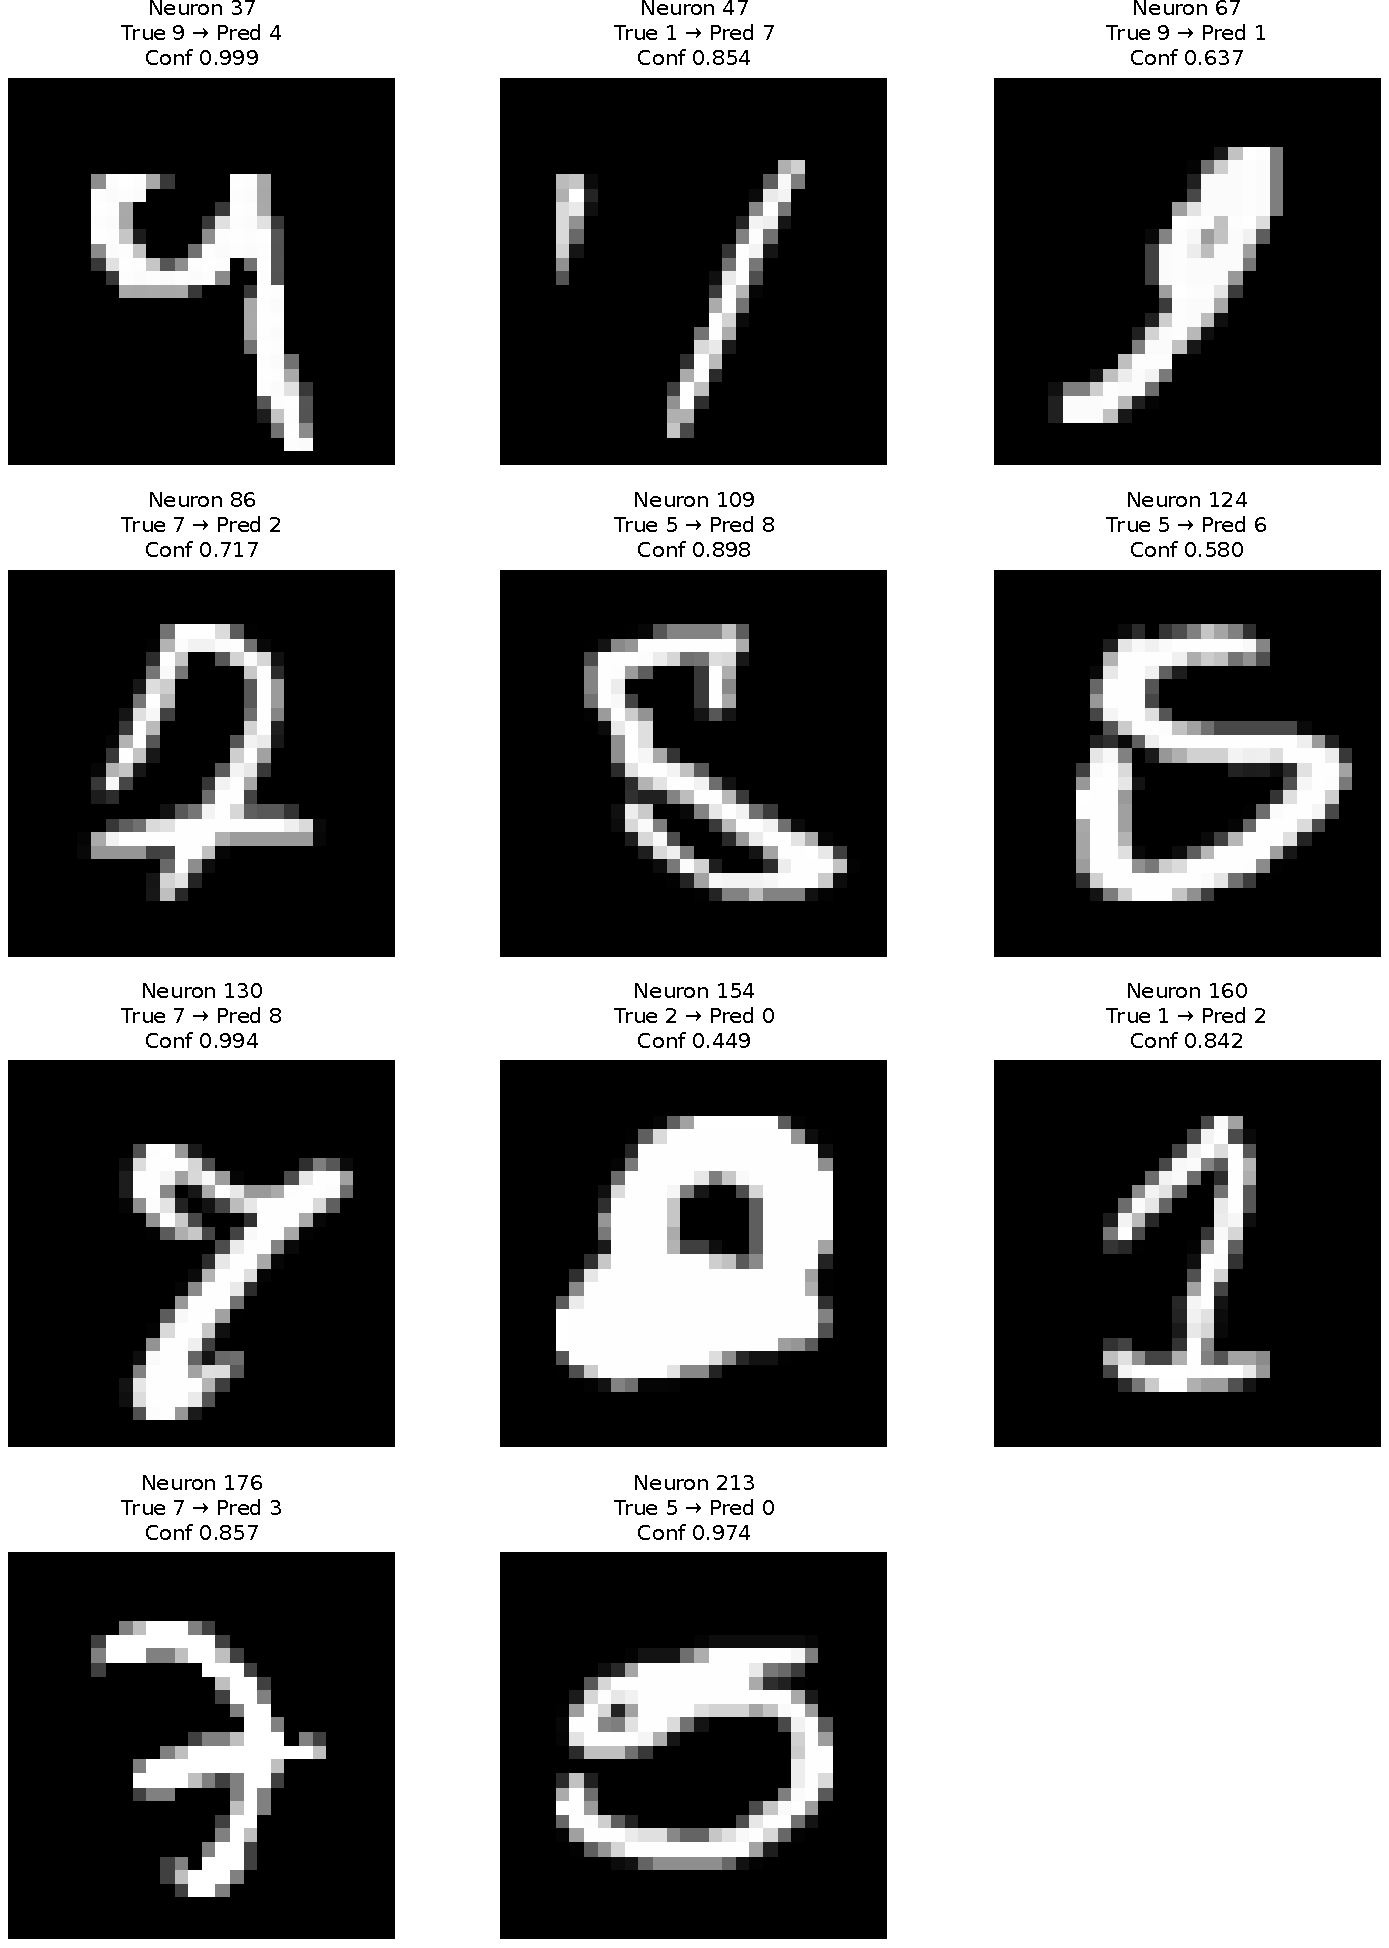
\includegraphics[width=0.8\linewidth,height=0.62\textheight,keepaspectratio]{hotspot_examples_mnist.pdf}
\caption{MNIST: one representative misclassification from each of the 11 hotspot cells (the validation error farthest from its cell), with its true class, predicted class and confidence.}
\label{fig:hotspot_mnist}
\end{figure}

\begin{figure}[htbp]
\centering
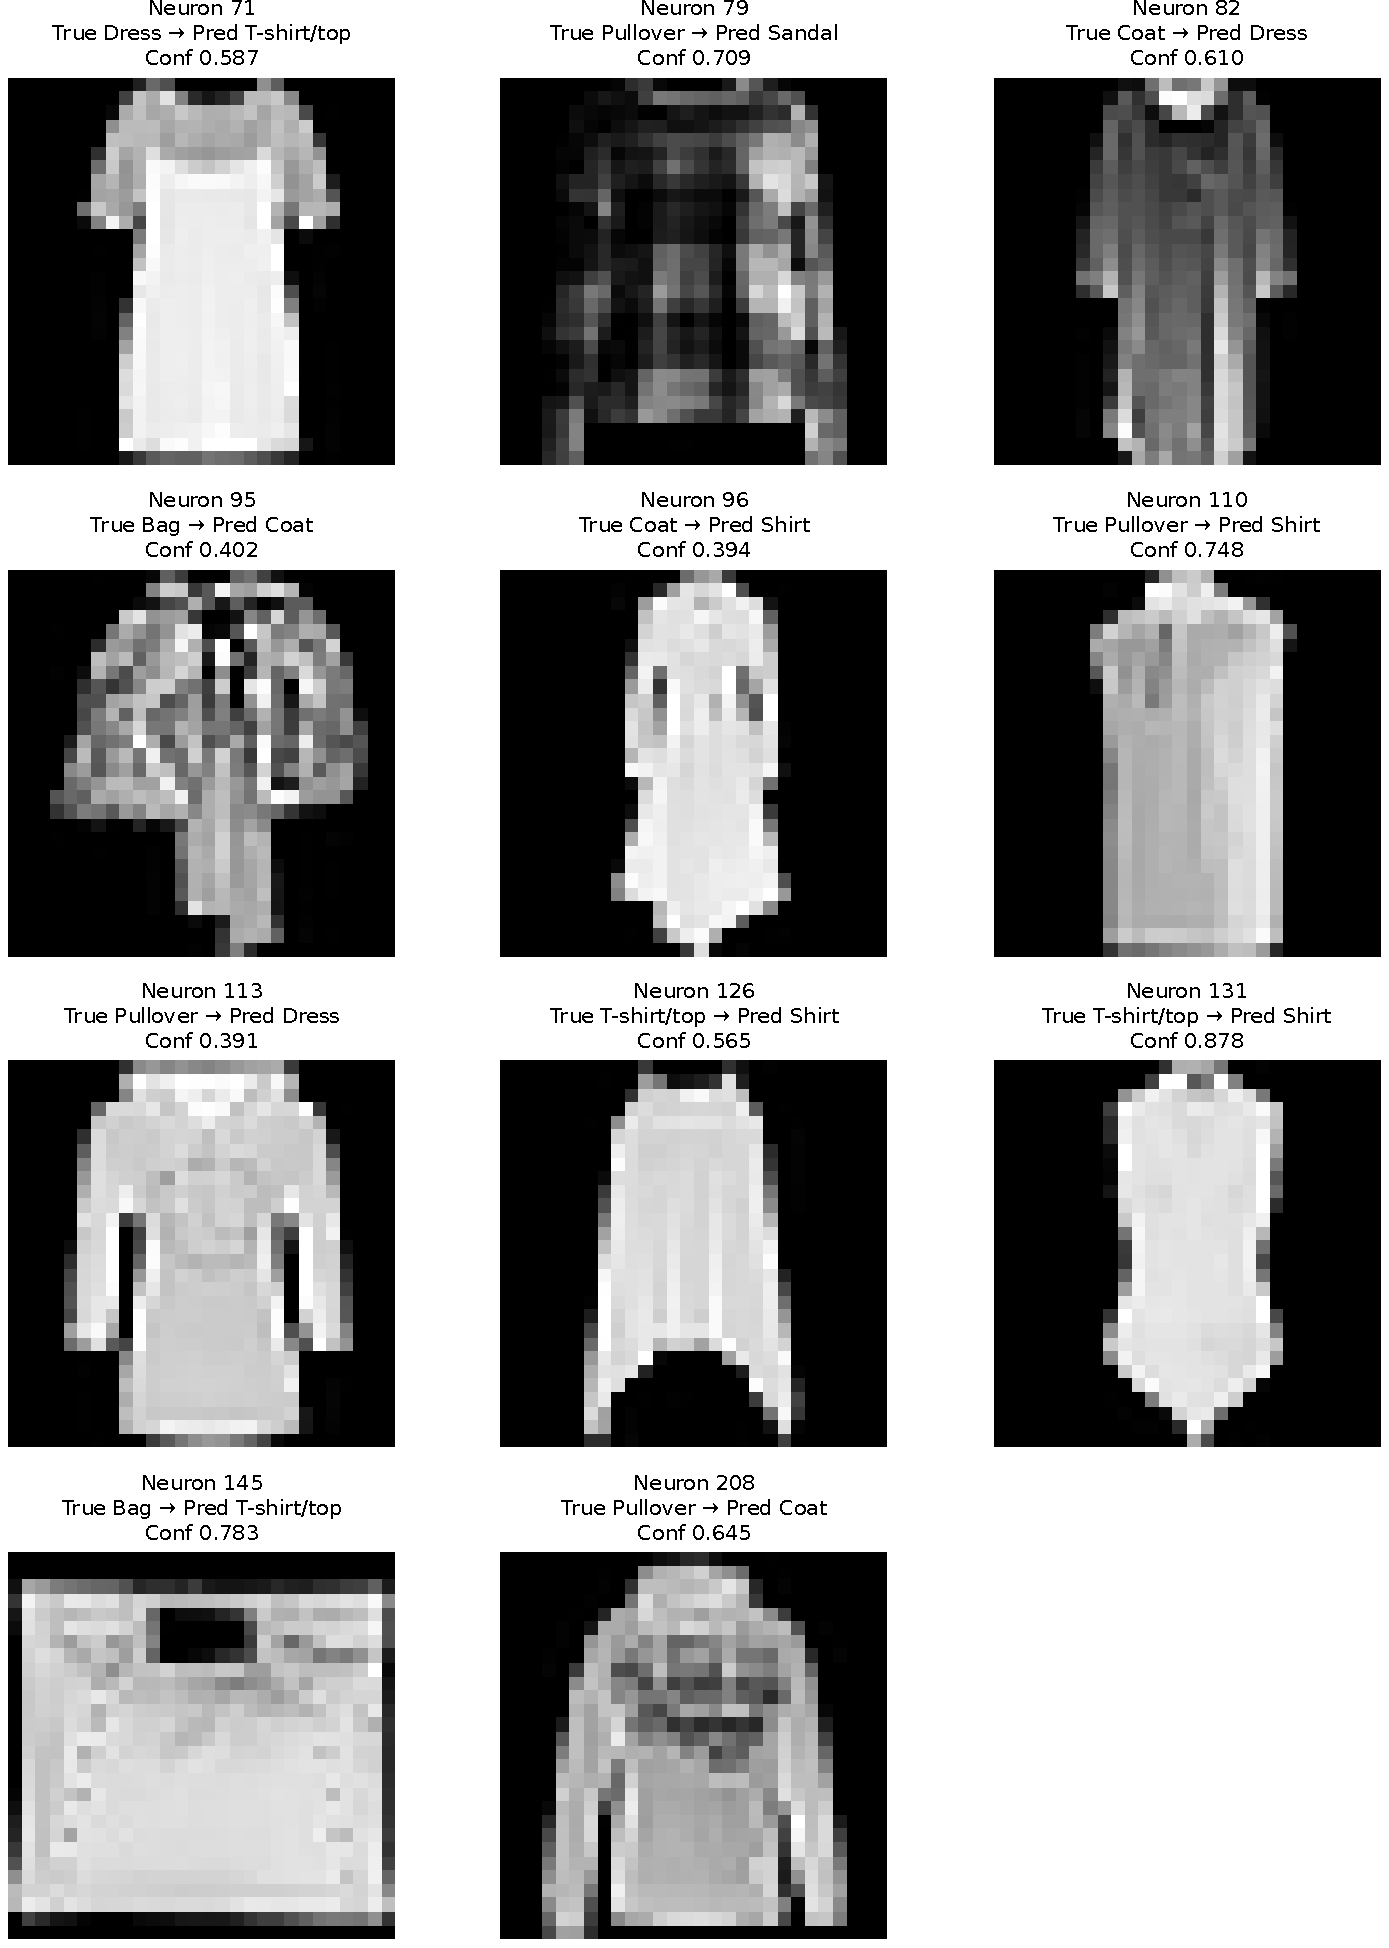
\includegraphics[width=0.8\linewidth,height=0.62\textheight,keepaspectratio]{hotspot_examples_fashion_mnist.pdf}
\caption{Fashion-MNIST: one representative misclassification from each of the 11 hotspot cells, as in Fig.~\ref{fig:hotspot_mnist}.}
\label{fig:hotspot_fashion}
\end{figure}

\FloatBarrier
\bibliographystyle{elsarticle-num}
\bibliography{references}

\end{document}
